\documentclass[11pt,harvard]{article}
\usepackage[letterpaper,top=1in, bottom=1in, left=1in, right=1in]{geometry}
\usepackage{graphicx}
\usepackage[sort]{natbib}
\usepackage{amssymb}
\usepackage{draftwatermark}
\SetWatermarkText{DRAFT - DO NOT SHARE \\	\\STRICTLY FOR INTERNAL USE}
\SetWatermarkFontSize{5cm}
\SetWatermarkScale{0.30}
\SetWatermarkColor[gray]{0.80}
\usepackage{amsmath}
\usepackage{setspace}
\usepackage{url}
\usepackage{pdflscape}
\usepackage{longtable}
\usepackage{threeparttable, booktabs}
\usepackage[export]{adjustbox}
\usepackage{enumitem}
\usepackage{comment}
\usepackage{subcaption}
\usepackage{lmodern}
\usepackage[T1]{fontenc}
\usepackage{setspace} % Load the setspace package
\usepackage{parskip} % Load the parskip package
\usepackage{float}
\usepackage{subcaption}
\usepackage{hyperref}
\usepackage[table,xcdraw]{xcolor}


\author{rCARI Study Team - WFP, ROME \\	\\For enquiries contact:\\		\\alirah.weyori@wfp.org, nicole.wu@wfp.org or mohamed.salem@wfp.org}
\date{\today}
\title{Validation and Calibration of the Remote Consolidated Approach of Reporting on Food Security (rCARI) Methodology 
	\\ {\normalsize Preliminary results from Myanmar, Ecuador, and Central African Republic}}


\begin{document}
	\maketitle \vspace{-1cm}
	\onehalfspacing
	\pagebreak
	\setlength{\parskip}{8pt} % Set the desired space before and after paragraphs
	
	\tableofcontents
	\pagebreak
	
	% -------	
	
\section{Executive Summary}

During the COVID-19 pandemic, there was an urgent need to develop a methodology to assess food security in a timely manner, without exposing enumerators to the risk of infection. The WFP thus developed and used quick and easy-to-administer questionnaires to assess the food security situation of the population over the phone. A remote version of the Consolidated Approach for Reporting Food Insecurity (rCARI) was developed as an adaptation of the standard CARI methodology to report on food insecurity. The rCARI method differed from the standard CARI only in the economic vulnerability dimension. While the standard CARI used food expenditure (FES) or economic capacity to meet essential needs (ECMEN) as an economic vulnerability indicator, rCARI used the household’s income source and income change in place of FES because of the difficulty of collecting expenditure data over the phone. Although the rCARI methodology is gradually gaining acceptance in most WFP country offices because of its ease of use, empirically, it has not yet been validated against the standard CARI.

Using a survey experiment methodology, this study validates the rCARI methodology of computing and reporting on food security with the standard CARI methodology. The study is being piloted across six countries in Africa, Latin America, the Middle-East, and Asia. The study sample frame is the national population from which a random sample of households were selected (except in Myanmar where because of accessibility issues the study was conducted among internally displaced persons (IDPs)) in at least 2 ADMIN1 areas involving between 20-25 ADMIN5 areas. Respondents were randomly enlisted into the study through a random walk in the village. Listed households were then randomly assigned to one of two study groups, the Face-to-Face (F2F ) group, which  received the standard CARI modules in a F2F interview or the Remote group, which received the rCARI interview by phone. The study has been implemented in three pilot countries so far – Myanmar (1,093 interviews in total), Ecuador (1,416 completed interviews), and Central African Republic (1,245 completed interviews), where data collection and analysis has been completed as of the end of August 2023. Data collection in the remaining three countries is expected to start soon.

Analysis of the data is premised on comparing different versions of CARI using remote or F2F modules. Three versions of CARI were then calculated and compared with the standard CARI. These include: 1) CARI using FES from remote surveys, 2.) CARI using the income variable from F2F surveys, and 3) CARI using income sources and income change variable from remote surveys (this is the version of CARI that was implemented at the height of the Covid pandemic).  Aside from the main comparison of CARI vs. rCARI, the study also compared different versions of the standard FES module (long vs. short versions) to consider implementation in remote surveys. There is also a comparison of LCS-FS vs LCS-EN modules.

The results of the study, though preliminary, show a number of interesting findings. The results of rCARI using the income \& income change indicator (rCARI-Inc) are not statistically different from the standard/conventional CARI (CARI-FES) in Myanmar \& Ecuador; however, it significantly underestimates food insecurity by 21 percentage points. Additionally, using the income source and income change indicator in place of the FES in F2F surveys would significantly underestimate food insecurity between 6\% to 22\% points. Thirdly, FCS, rCSI, FES and income sources indicators collected over phone tend to give similar or slightly different results than in F2F data collection, with differences in FCS (0 to 8 points), rCSI (-1 to 4 points) FES (5\% - 8\% points), and income sources (0 to 8\% points in category 4 ) (1\% to 11\% points in category 3). Fourth, administering the LCS module in its current form over the phone is problematic and may need further refinement and enumerator training. However, in terms of testing the different versions of modules (LCS-FS vs. LCS-EN), the results show that there are no statistically significant differences.
 
Though in the early stages as yet in terms of the validity or otherwise of rCARI, a number of conclusions have been made based on the results thus far. First , conventional rCARI (income) largely under reports FI (food insecurity).  Second, almost all food security indicators are largely comparable between F2F and Remote modalities (where different, it is minimal). Third, food insecurity estimated using the FES indicator as an absolute value is always higher compared to the income indicator regardless of modality of data collection and thus replacing FES with the income indicator will lead to significantly lower acute food insecurity numbers. 

In the next steps, further in-depth analysis of the data collected will be conducted to better understand and standardize the income source and income change indicator to be used in food security assessments and reporting.


\pagebreak
	
% ------- 
	\section{Introduction}

Food security assessment and reporting are at the core of WFP’s mandate of addressing hunger and food insecurity. Over time, different methodologies (e.g., IPC, CARI, Cadre Harmonise, etc.) have been developed and used to assess and report global food insecurity each differing in scope, and purpose. A commonality that cuts across all methods is the use of primary household data collected through face-to-face interviews/surveys. However, in recent times particularly with the outbreak of the Covid-19 pandemic and attendant restrictions on movement and physical contact, data collection through conventional face-to-face method has been adversely affected. This impacted negatively the ability to assess food security needs because of the data gap created. Developing methodologies to accurately measure and interpret food insecurity especially in emergencies where physical access is restricted thus, is of great importance for WFP and many stakeholders. This is particularly important during emergencies when rapid assessment is required for advocacy to save lives and livelihoods but physical access to the field is restricted either because of health threats or security considerations for enumerators. 

To leverage the increased penetration of technology in operational areas of WFP during the Covid lockdowns, a remote version of the Consolidated Approach for Reporting Food Insecurity (CARI)- the so-called rCARI- was developed as an adaptation of the standard CARI methodology and administered remotely (over the phone). The methodology though viewed favourably by researchers, and the larger humanitarian community, because of the stop-gap solution it provided during the covid-19 lockdown, questions about the validity of food security numbers it produces remain. For example, how are the remote modules comparable with already standardized face-to-face modules in capturing food insecurity. Although there exist validated studies on the use of face-to-face modules in assessing and reporting on food insecurity, remote methodology such as rCARI remains scant until now. 

The potential advantages of the methodology abound for humanitarian work particularly for hard-to-reach areas. For example, the remote methodology has potential to save lives by providing real-time food insecurity data on the exposed population within the shortest possible time to inform policy. Furthermore it can result in better use of scarce resources to achieve high end results by rolling out few targeted modules to assess food insecurity of a larger population.  	

The overall goal of this study was to assess the validity of the rCARI module(s) against conventional CARI modules for measuring food security within the same population. The study compares indicators collected through phone surveys with conventional face-to-face surveys, considering the latter as the standard methodology. The following food security indicators were compared: Food Consumption Score (FCS), reduced Coping Strategy Index (rCSI), Livelihood Coping Strategy (LCS), Food Expenditure Share (FES), and income sources and income change. The Economic Capacity to Meet Essential Needs (ECMEN) indicator, which is recommended to be used to calculate CARI will not be tested in this study, as it requires a standard long expenditure module, which cannot be collected over phone. In addition, ECMEN calculation requires having an updated value of the minimum expenditure basket (MEB) of the study population, which is not available for some of the study areas. Instead, a shortened version of the standard expenditure module will be used to test the possibility of collecting FES data over the phone.

Studying the validity of using the phone to collect food security indicators is a key step in judging the appropriateness of the rCARI methodology to report food insecurity prevalence. However, testing the comparability of these indicators through different modalities of data collection (Face- to-Face (F2F) vs. Phone) should be read within the wider consideration around phone survey modality of data collection. For example, other factors aside from the modules should be considered while reading the results of any remote survey.
	
	\begin{itemize}[label=--, left=1.5em]
		\item[1.]	Mobile phone ownership (mobile phone penetration rate in the study area) could likely exclude the most vulnerable population from the sample. 
		
		\item[2.]	Mobile phone network coverage; Even in countries with high penetration rates, network coverage could be a problem, especially when electricity cuts are frequent and local infrastructure, such as communication masts, are not evenly distributed (World Bank, 2020).
		
		\item[3.]	Response rate: It is well documented that the response rate in phone surveys is usually lower than in face-to-face surveys (L’Engle et al., 2018; World Bank, 2020). 
	\end{itemize}
	
Nevertheless, there are several statistical weighting techniques that can adjust the results of phone surveys based on baseline variables like demographics characteristics of the most recent face-to- face surveys (Nagpal et al. 2021; Glazerman et al. 2020; Valliant et al. 2013; Elkasabi, 2015). This allows the final results of such exercises to be aggregated and extrapolated to reflect some level of representativeness. 

However, this current study may not be affected by these confounding issues since the main idea is not to report the results at the national level but rather to evaluate the effectiveness of the remote modules in collecting and reporting on food security. For this reason, the study does not focus on weighting techniques to adjust for sampling skewness and response rate. Nonetheless, the study design adopted in Central African Republic (CAR), could allow for testing of sample skewness due to mobile phone ownership and coverage (see CAR sample design in Annex). CAR has one of the lowest mobile phone penetration rates globally (approximately 70\% of the population do not own mobile phones).
	
\pagebreak
	
% ------- 
	
\section{Study design}
	
The study was implemented as a survey experiment with stratified sample of respondents who are randomly selected to two groups; CARI Group (F2F) and rCARI Group (Remote). The study designed followed rigorous randomization procedures to assign potential respondents to the study groups to ensure statistical comparability of the two sub-samples. For a systematic household/respondent selection process, refer to Figure 1. 
	
\begin{figure}[H]
		\begin{center}
			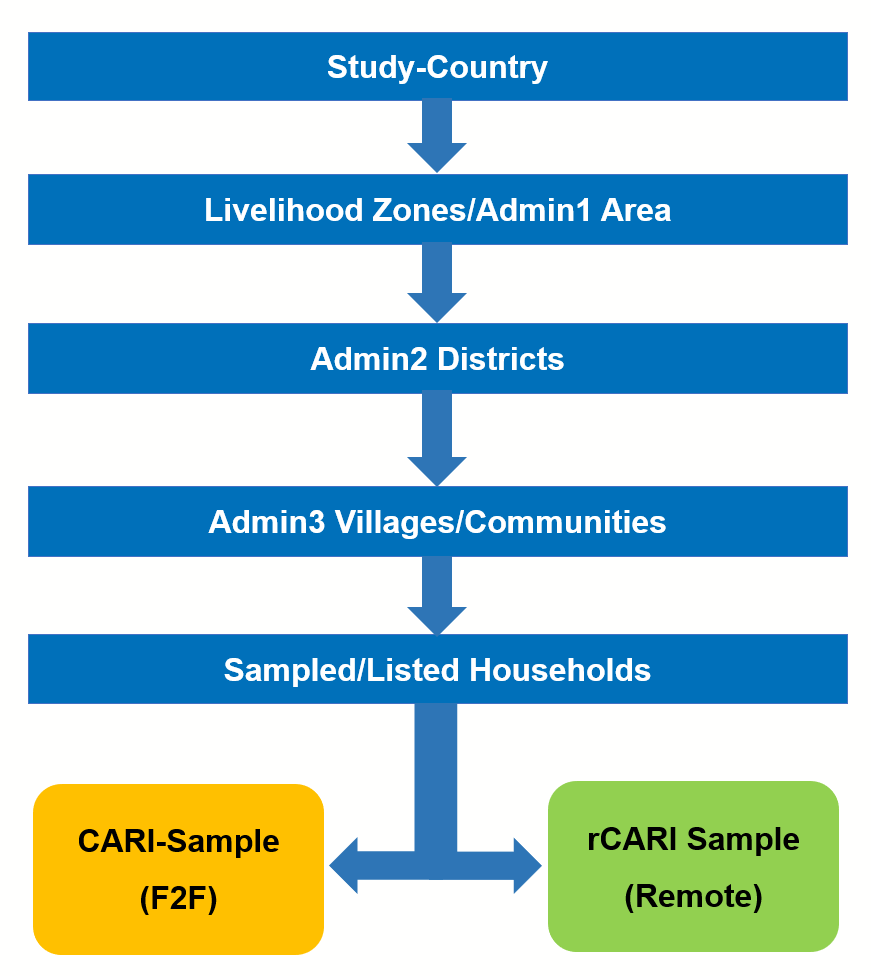
\includegraphics[scale=.65]{2_figure/Sample_Frame.png}
		\end{center}
		\label{fig:Sample_Frame}
		\caption{rCARI Validation Study Sampling Frame}
	\end{figure}
	
\begin{itemize}[label=--, left=1.5em]
	\item[1.] STEP 1 - Livelihood Zones/ADMIN1 Area Selection: A minimum of 2/3 Admin1 Areas were identified together with WFP CO based on phone coverage, food security situation and accessibility. If more than 3 Admin1 areas met the criteria, a simple random approach was used to select the required number of Admin1 Areas.
		
	\item[2.] STEP 2 - ADMIN2 Selection: A minimum of 4 ADMIN2 areas were randomly selected (2 per ADMIN1 Area based on the outcome of Step 1). 
		
	\item[3.] STEP 3 - ADMIN5 (villages, communities or camps) Areas: All ADMIN 5 (villages) in ADMIN2 that meets the inclusion criteria set out in STEP 1 are now compiled at this stage as the primary sampling units (PSUs). A total of 20 PSUs were randomly selected (distributed uniformly across the selected ADMIN1 AREAS) as sampling clusters to draw the households from. 
		
	\item[4.] STEP 4 - Sampled households: The sampling frame for the study was all households in selected PSUs. A minimum of 100 households per PSU were selected through the random-walk approach (listing every 3rd house in the sequence) by trained enumerators. Consent of participation was taken from all HHs before being included into the study sample. Based on the number of PSUs per country, 2,000-2,500 HHs (except in Myanmar where the initial sample was 1,665HHs). The final listed households in this stage were used for the randomization process in the next step.
		
	\item[5.] STEP 5 - Randomization of household (hh): Consented final sampled households in STEP 4 are randomly assigned into one of two survey modalities/groups; F2F (CARI group) and Remote (rCARI group). The designed is programmed such that sample will be divided equally between the modalities. All interviews were conducted over the same time frame to ensure that households in the two modalities are reporting their food security situation over the same window. 
		
\end{itemize}
	
After the randomization was done (STEP 5), using baseline household and respondents collected during the listing phase, a statistical balance of the two groups is done. This is to ensure that the two study groups are statistically comparable. Food security data was collected using standardized face-to-face and remote modules administered to the two groups collecting household level food security indicators. 
	
The study is being implemented across six countries: 2 in Africa, 2 in Latin America, 1 in Southeast Asia, and 1 in the Middle East. After the first round of data collection covering the period May 2023 to August 2023, surveys in Myanmar, Ecuador and CAR involving approximately 3,755 households have been completed. The remaining 3 countries are planned to start soon.
	
	\subsection{Selection of study areas and participants}
	
Survey participants were enlisted into the study through a stratified random process. A minimum of 100 potential participating households were enlisted per Admin5 area (except for Myanmar where the study was conducted amongst 20 IDP camps and some of the camps had fewer than 100 households). The listed households formed the sampling frame for the group/modality assignment which was then done randomly. 
	
In the listing phase of the study, baseline variables that included demographic characteristics of potential respondents and their households was collected in Ecuador and CAR. This was not possible in Myanmar because field access restrictions. The initial sample size listed for the study was 1665 households in Myanmar, 2372 households in Ecuador, and 2500 households in CAR. 
	
	
	\subsection{Myanmar}
	
The study in Myanmar was implemented in two regions: Kachin and Shan (Admin 1). The sampling list was compiled using WFP beneficiaries made up of internally displaced persons (IDPs) in the two regions. Phone ownership was a key criterion for inclusion in the study. However, being WFP beneficiaries, all participants in Myanmar owned phones. A total of 20 camps were selected as the primary sampling units (PSU), respondents/households were then randomly selected and used in the randomization stage.

Data collection was conducted by WFP field staff after a 3-day training that was led by the WFP Regional Bureau of Bangkok in collaboration with the Myanmar CO and supported by the rCARI study team from HQ.  The training and data collection were administered in Burmese, the official language of Myanmar. 

A total of 610 (73\%) household interviews were completed for the F2F modality, while 483 (58\%) households were interviewed by phone (remote modality). A balance test of the randomization indicated that the baseline household characteristics were well balanced between the two groups (modalities). 
	
	\subsection{Ecuador}
	
In Ecuador, the study was implemented in three regions: Amazonia, Coasta and Sierra (Admin1 areas). In addition to the standard selection criteria based on accessibility and food security prevalence, consideration was also given to the safety of the team, considering the political upheaval at the time of implementing the study. A total of 27 Admin5 areas (villages) were randomly selected from these 3 Admin1 areas.

The sampling frame was all households in the 23 ADMIN5 areas that had been randomly selected to participate in the study. The study sample was enlisted following a random walk in each of the Admin5 areas and selecting every 3rd household. Demographic characteristics as well as contact details including the phone number of the household head was then collected at this stage (listing phase). Contact details for a  total of 2,374 households were collected  after receiving written consent. Since households may be interviewed by phone, potential respondents  or someone within the household had to own a phone through which they may be contacted for the survey. Households that were selected but had no phone, were eliminated, and replaced by the next household on the list. This was, however, observed to be minimal in Ecuador because of the high national mobile phone penetration 80\% (see Figure 2 for the sample distribution and levels of randomization).

Enumerator training was jointly conducted by the Ecuador CO and the Regional Bureau of Panama (RBP) colleagues in Spanish over a 4-day period with a one-day simulation for remote and F2F instruments. Interviews were conducted in Spanish, the official language of Ecuador. The field work in Ecuador took place between June and July 2023. 

\begin{figure}[H]
		\begin{center}
			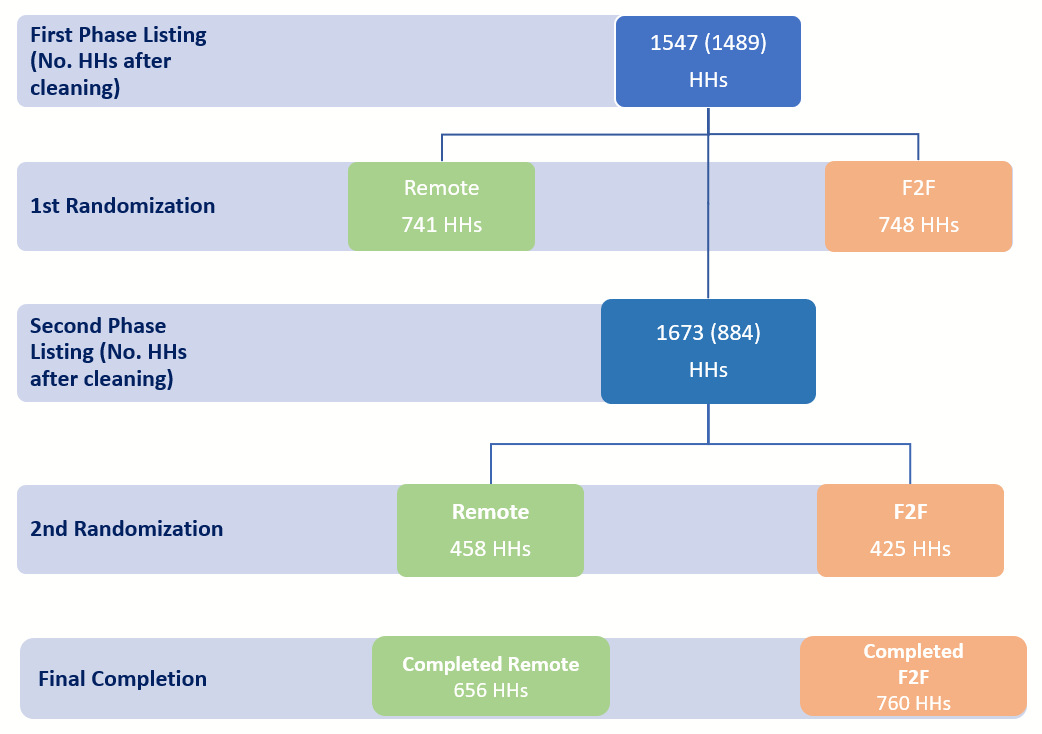
\includegraphics[scale=.65]{2_figure/Ecuador_Sample_Composition.png}
		\end{center}
		\caption{Sample Composition and Completion in Ecuador}
		\label{fig:Ecuador_Sample_Composition}
	\end{figure}
	
	
	\subsection{Central African Republic}
	
The study in CAR was implemented in 2 prefectures - Mbomou and Nana-Gribizi (Admin1), the two most accessible areas (aside from Bangui) that also had a varying level of food security. The selection of PSUs followed a similar pattern using field access (security situation) and mobile phone network coverage. The list of Admin5 areas that met the access and mobile phone coverage criteria formed the sampling frame. A total of 25 Admin5 areas (villages) were randomly selected from the list of Admin5 areas compiled jointly by the CAR CO and the local mobile phone service providers (to ensure that all Admin5 areas selected had mobile phone network). Admin5 areas without phone coverage were automatically excluded.
To ensure that the final sample was a mix of rural and urban households (taking into consideration there was a potentially different food security situation between rural and urban households), sub layer of locality was included during the selection of Admin5 areas so that the final sampled villages was made up of rural and urban areas. Implementation of the household listing and survey was led by ICASES, the National Statistical Office of CAR.

The sampling frame for the study was all households in the 25 selected ADMIN5 areas. The listing phase was conducted through the random-walk methodology in each selected PSU by trained enumerators. 

A minimum of 100 households/respondents per PSU totaling 2500 households/respondents were listed as potential study participants. Phone numbers of the main respondent and any other phone numbers within the household that could have been used to contact the main respondent during the survey was collected. Drawing from the data collection experience in Myanmar and Ecuador, a number of demographic characteristics such as age of household head, gender of household head, household size, and ownership of common household assets was collected during household listing and used for the statistical balance test.

Training of enumerators was conducted  facilitators from the Regional Bureau of Dakar, and HQ with the support from the CAR CO. The training was conducted in French over a in 4-day period, including one day used for field testing, adjusting and adapting the final questionnaires (F2F \& Remote) before deployment for data collection. While the  enumerator training was conducted largely in French (except of the simulation), deployment for the actual field work was done systematically by the CO and ICASES so that each enumerator was sent to localities where they could speak the local dialects in case a respondent does not speak French thus require the interview is conducted in the local Sango dialect.
 
A large proportion of the population of CAR (approximately 70\%) do not own mobile phones. To ensure that the study compared appropriate households in terms of phone ownership and coverage, a slightly different sampling and randomization methods were applied  (see Figure 2 for all the sampling and randomization stages adopted in CAR). This allowed a segregation of phone-owners and non-phone-owners so that the results are not only compared by modality but also by phone-ownership. A statistical balance test between the different groups showed that respondents were significantly balanced (see Annex  for details).
	
\begin{figure}[H]
		\begin{center}
			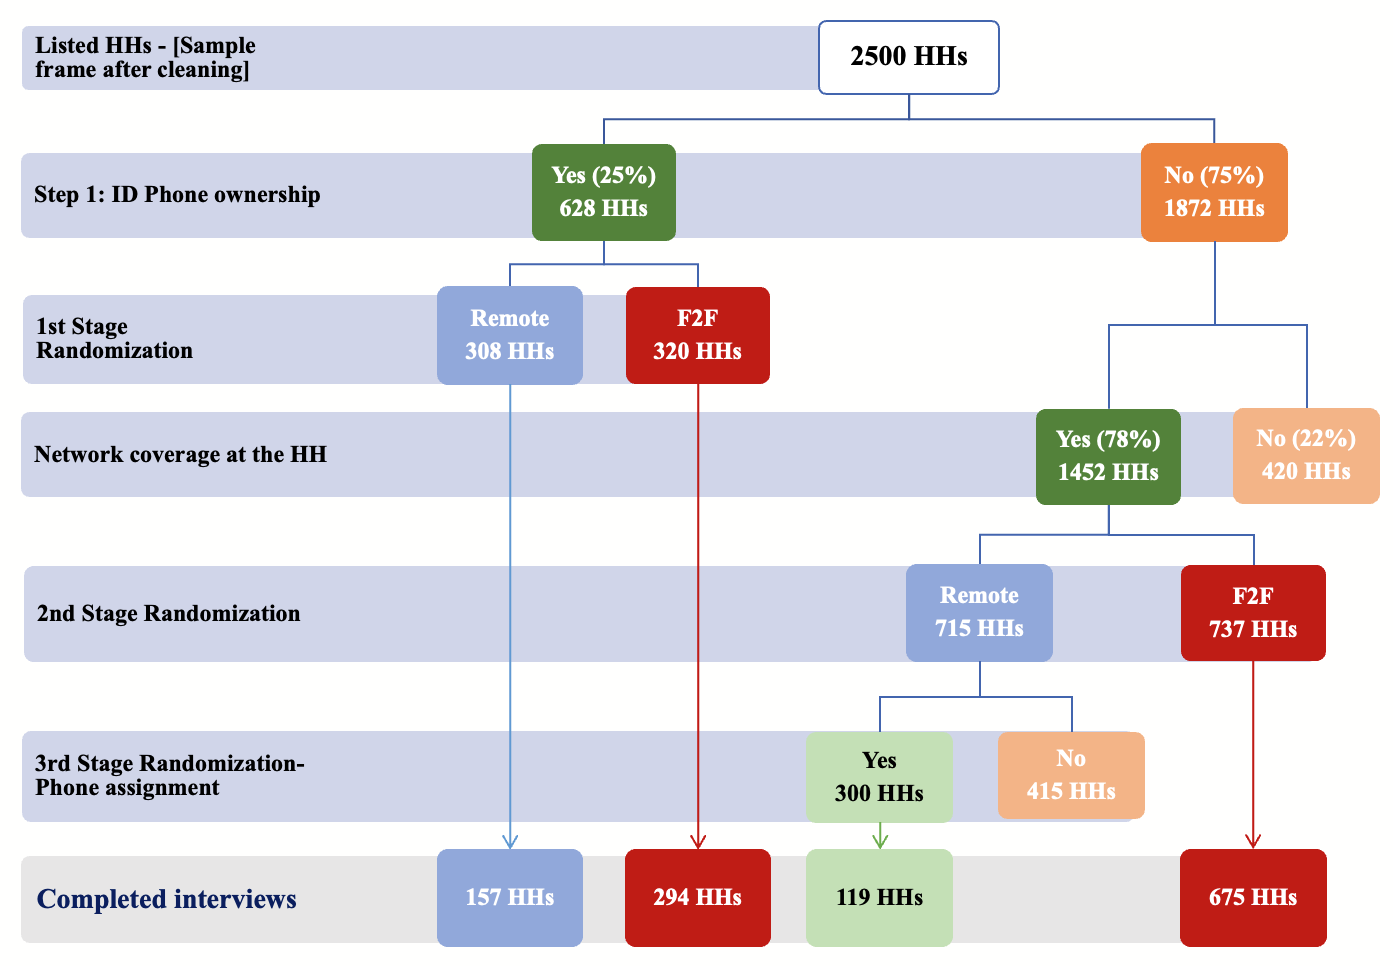
\includegraphics[scale=0.25]{2_figure/CAR_Sample_Composition.png}
		\end{center}
		\label{fig:CAR_Sample_Composition}
		\caption{Sample Composition and Completion in CAR}
	\end{figure}
	
	
	\subsection{Overall study implementation}
	
Data collection for both modalities was done simultaneously to cover the same period. The fieldwork was originally planned over a 3-week period (covering 1 week for enumerator training, adjusting questionnaire and 2 weeks for actual household interviews) in each pilot country. However, due to unforeseen challenges, data collection was extended by between 2 to 3 weeks in each country. See Figure 4 on the study implementation.
	
\begin{figure}[H]
		\begin{center}
			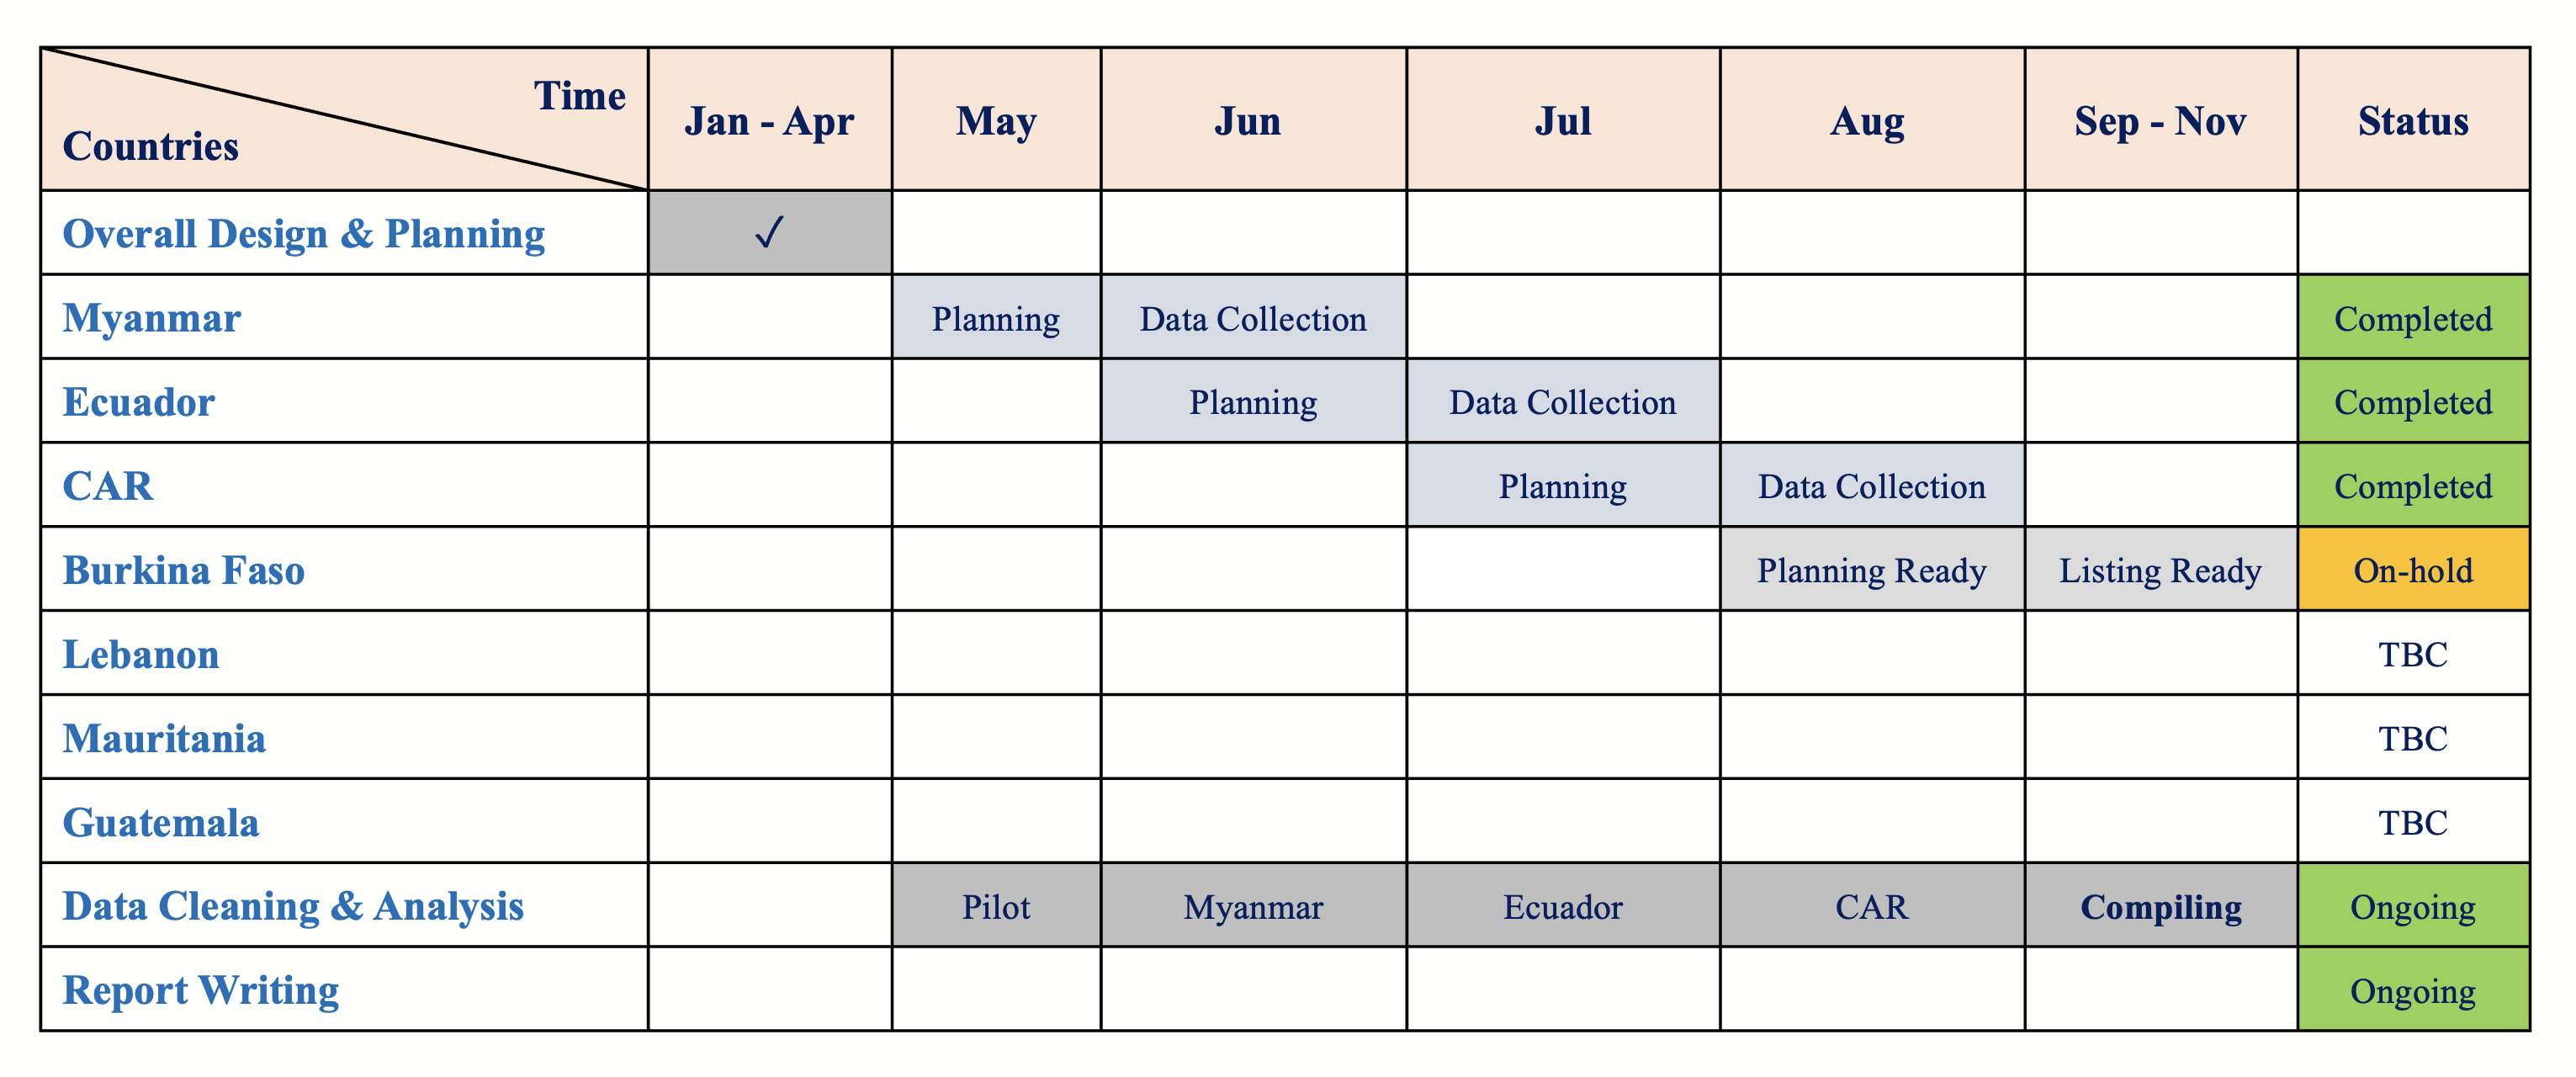
\includegraphics[scale=.3]{2_figure/Workplan.png}
		\end{center}
		\label{fig:Workplan}
		\caption{rCARI Validation Study Timelines \& Potential Pilot Countries}
	\end{figure}
	
In the next section, sample completion and initial results are presented for all countries completed at this stage of the study.
	

	\subsection{Sample Completion}
	
Table 1 shows the total sample and number of household interviews completed by country and modality in the initial 3 pilot countries of the study.
	
	\begin{table}[!h]
\caption{Survey Completion by Country}
\centering
\begin{tabular}{lllll}
\cline{1-5}
\multicolumn{1}{r}{} &
  \multicolumn{4}{c}{Country} \\
\multicolumn{1}{r}{} &
  \multicolumn{1}{c}{Myanmar} &
  \multicolumn{1}{c}{Ecuador} &
  \multicolumn{1}{c}{CAR} &
  \multicolumn{1}{c}{Total} \\
\cline{1-5}
\multicolumn{1}{l}{N} &
  \multicolumn{1}{r}{1,665 (27.2\%)} &
  \multicolumn{1}{r}{2,372 (38.8\%)} &
  \multicolumn{1}{r}{2,080 (34.0\%)} &
  \multicolumn{1}{r}{6,117 (100.0\%)} \\
\multicolumn{1}{l}{Survey Progress} &
  \multicolumn{1}{r}{} &
  \multicolumn{1}{r}{} &
  \multicolumn{1}{r}{} &
  \multicolumn{1}{r}{} \\
\multicolumn{1}{l}{\hspace{1em}Not Completed} &
  \multicolumn{1}{r}{572 (34.4\%)} &
  \multicolumn{1}{r}{956 (40.3\%)} &
  \multicolumn{1}{r}{835 (40.1\%)} &
  \multicolumn{1}{r}{2,363 (38.6\%)} \\
\multicolumn{1}{l}{\hspace{1em}Completed} &
  \multicolumn{1}{r}{1,093 (65.6\%)} &
  \multicolumn{1}{r}{1,416 (59.7\%)} &
  \multicolumn{1}{r}{1,245 (59.9\%)} &
  \multicolumn{1}{r}{3,754 (61.4\%)} \\
\multicolumn{1}{l}{Survey Modality} &
  \multicolumn{1}{r}{} &
  \multicolumn{1}{r}{} &
  \multicolumn{1}{r}{} &
  \multicolumn{1}{r}{} \\
\multicolumn{1}{l}{\hspace{1em}Face-to-Face} &
  \multicolumn{1}{r}{610 (55.8\%)} &
  \multicolumn{1}{r}{760 (53.7\%)} &
  \multicolumn{1}{r}{969 (77.8\%)} &
  \multicolumn{1}{r}{2,339 (62.3\%)} \\
\multicolumn{1}{l}{\hspace{1em}Remote} &
  \multicolumn{1}{r}{483 (44.2\%)} &
  \multicolumn{1}{r}{656 (46.3\%)} &
  \multicolumn{1}{r}{276 (22.2\%)} &
  \multicolumn{1}{r}{1,415 (37.7\%)} \\
\cline{1-5}
\end{tabular}
\end{table}
 
	\label{tab:rCARI_Overall_Completion}
	
As expected, the response rate in the remote sample was lower than the F2F in all three countries. This was primarily due to the poor phone connection/network and not picking up the  phone calls, with less than 1\% of all calls refusals to be interviewed. Nevertheless, this did not influence the sample balance for almost all the collected background information at the household level for Ecuador and Myanmar. 
In CAR, however, the study sample was sub-categorized into phone-owners and non-phone-owners to capture phone and network coverage differences. The balance test performed showed that the two samples were largely balanced over the two modalities. For more details about response rate, the final sample statistical balance analysis test (see attrition tables attached in Annex).
	
	
\pagebreak
	
% ------- 
	\section{Results and Discussions}
	
This section presents the main results of the study by the food security indicators, testing their comparability conducting group mean test (student t-test). Here, the objective is to compare the different versions of CARI calculated either using remote or face-to-face modules with the standard CARI.
	
\subsection{CARI vs. rCARI}
	
Here, the standard CARI using FES from F2F surveys was compared to other ways of aggregating CARI (below and in Table 2):
	
	Other ways of aggregating CARI (that are tested)
	\begin{itemize}[label=--, left=1.5em]
		\item rCARI-FES: Standard CARI using FES from remote surveys.
		\item CARI-Inc: CARI using income variable from F2F surveys.
		\item rCARI-Inc: Standard rCARI using income and income change variable from remote surveys (the CARI version that was used during COVID 19 Pandemic).
	\end{itemize}
	
For the purposes of this interim analysis and report, results from  CAR are restricted to only respondents that owned phones (the complete sample comprising those who did not own phones but received mobile phones from the study are  also available).
	
	\begin{table}[htbp]
		\centering
		\begin{adjustbox}{max width=\textwidth}
			\begin{threeparttable}
				\caption{Lists the different aggregation methods and indicators used for each methodology}
				\scriptsize
				\begin{tabular}{lcccc}
	\hline
\multicolumn{1}{c}{\textbf{}}           & \multicolumn{4}{c}{\textbf{Aggregation Methodology}}                                                                                                                                                                                                                     \\ \hline
\textbf{Indicator}                      & \textbf{\begin{tabular}[c]{@{}c@{}}CARI\\ (F2F)\end{tabular}} & \textbf{\begin{tabular}[c]{@{}c@{}}CARI \\ (F2F)\end{tabular}} & \textbf{\begin{tabular}[c]{@{}c@{}}rCARI \\ (Remote)\end{tabular}} & \textbf{\begin{tabular}[c]{@{}c@{}}rCARI \\ (Remote)\end{tabular}} \\
\textbf{FCS}                            & Yes                                                           & Yes                                                            & Yes                                                                & Yes                                                                \\
\textbf{FES}                            & Yes                                                           & {\color[HTML]{CB0000} \textbf{No}}                             & Yes                                                                & No                                                                 \\
\textbf{LCS}                            & Yes                                                           & Yes                                                            & Yes                                                                & Yes                                                                \\
\textbf{rCSI}                           & Yes                                                           & Yes                                                            & Yes                                                                & Yes                                                                \\
\textbf{Income source \& income change} & {\color[HTML]{CB0000} \textbf{No}}                            & Yes                                                            & {\color[HTML]{CB0000} \textbf{No}}                                 & {\color[HTML]{CB0000} \textbf{Yes}}                               \\ \hline
\end{tabular} 
				\label{tab:Aggregation_Table}
			\end{threeparttable}
		\end{adjustbox}
	\end{table}
	
For more information on the calculation of the food security indicators included in each methodology refer to supporting documents attached in the Annex. 
	
The first comparison is between rCARI-Inc  (using the income and income change variable) with standard CARI presented in Table 3 for all of the pilot countries. In Myanmar and Ecuador, there was no statistically significant differences reported in the prevalence of food insecurity (moderately food insecure plus severely food insecure) between the two aggregation methodologies. However, in CAR, rCARI-Inc underestimated the prevalence of food insecurity by 21 percentage points compared to CARI-FES. Further, rCARI-Inc was identical to CARI-FES in estimating the percentage of moderately food insecure in Myanmar and Ecuador but underestimated. 

In CAR, rCARI-Inc significantly underestimated the moderately food insecure numbers and severely food insecure by 15 and 6 percentage points, respectively, compared to CARI-FES.
	
	\begin{table}[htbp]
		\centering
		\begin{adjustbox}{max width=\textwidth}
			\begin{threeparttable}
				\caption{Impact of Survey Modality: Standard CARI-FES vs. Standard rCARI-Inc}
				\scriptsize
				\begin{tabular}{l*{9}c}
\hline\hline
 & \multicolumn{3}{c}{Myanmar} & \multicolumn{3}{c}{Ecuador} & \multicolumn{3}{c}{CAR}\\ 
Variable & F2F & Remote & Diff & F2F & Remote & Diff & F2F & Remote & Diff \\
\hline
Food Secure&0.08&0.07&-0.01&0.01&0.00&-0.01&0.01&0.01&-0.00\\
&(0.27)&(0.26)&(0.67)&(0.11)&(0.07)&(0.08)&(0.08)&(0.08)&(0.96)\\
Marginally Food Secure&0.44&0.41&-0.03&0.23&0.27&0.03&0.31&0.52&0.21***\\
&(0.50)&(0.49)&(0.42)&(0.42)&(0.44)&(0.13)&(0.46)&(0.50)&(0.00)\\
Moderately Food Insecure&0.44&0.49&0.05&0.59&0.62&0.03&0.60&0.45&-0.15**\\
&(0.50)&(0.50)&(0.23)&(0.49)&(0.48)&(0.22)&(0.49)&(0.50)&(0.00)\\
Severely Food Insecure&0.03&0.03&-0.01&0.16&0.11&-0.06**&0.08&0.02&-0.06**\\
&(0.18)&(0.16)&(0.59)&(0.37)&(0.31)&(0.00)&(0.27)&(0.14)&(0.00)\\
Food Insecure Group&0.47&0.51&0.04&0.76&0.73&-0.03&0.68&0.47&-0.21***\\
&(0.50)&(0.50)&(0.31)&(0.43)&(0.44)&(0.26)&(0.47)&(0.50)&(0.00)\\
\hline
Observations & 610 & 232 & 842 & 760 & 656 & 1,416 & 294 & 157 & 451 \\
\hline\hline
\end{tabular}
 
				\label{tab:CARI_rCARI_Modality_All_Country}
				\begin{tablenotes}[para,flushleft]
					\item Note: Robust standard errors in parentheses; * p$<$0.05, ** p$<$0.01, *** p$<$0.001. 
				\end{tablenotes}
			\end{threeparttable}
		\end{adjustbox}
	\end{table}
	

Table 4 shows the results of rCARI calculated using the FES collected by phone and represents the scenario of collecting all CARI indicators over phone in remote interviews. As discussed earlier, the FES collected over the phone is a relatively shorter version of the standard FES that is usually collected in F2F surveys. This version collects the household’s aggregate expenditures without going into the individual expenses. The results show that rCARI using FES consistently over-estimates the number of food insecure across all countries compared to the standard CARI by between 2 and 17 percentage points. This difference was statistically significant in Myanmar and Ecuador.

	\begin{table}[htbp]
		\centering
		\begin{adjustbox}{max width=\textwidth}
			\begin{threeparttable}
				\caption{Impact of Survey Modality: CARI-FES vs. rCARI-FES}
				\scriptsize
				\begin{tabular}{l*{9}c}
\hline\hline
 & \multicolumn{3}{c}{Myanmar} & \multicolumn{3}{c}{Ecuador} & \multicolumn{3}{c}{CAR}\\ 
Variable & F2F & Remote & Diff & F2F & Remote & Diff & F2F & Remote & Diff \\
\hline
Food Secure&0.08&0.03&-0.06***&0.01&0.00&-0.01**&0.01&0.01&-0.00\\
&(0.27)&(0.16)&(0.00)&(0.11)&(0.04)&(0.01)&(0.08)&(0.08)&(0.96)\\
Marginally Food Secure&0.44&0.34&-0.10**&0.23&0.07&-0.16***&0.31&0.29&-0.02\\
&(0.50)&(0.48)&(0.01)&(0.42)&(0.26)&(0.00)&(0.46)&(0.45)&(0.61)\\
Moderately Food Insecure&0.44&0.57&0.13***&0.59&0.69&0.10***&0.60&0.58&-0.02\\
&(0.50)&(0.50)&(0.00)&(0.49)&(0.46)&(0.00)&(0.49)&(0.50)&(0.65)\\
Severely Food Insecure&0.03&0.06&0.02&0.16&0.23&0.07**&0.08&0.13&0.05\\
&(0.18)&(0.23)&(0.17)&(0.37)&(0.42)&(0.00)&(0.27)&(0.33)&(0.14)\\
Food Insecure Group&0.47&0.63&0.16***&0.76&0.92&0.17***&0.68&0.71&0.02\\
&(0.50)&(0.48)&(0.00)&(0.43)&(0.27)&(0.00)&(0.47)&(0.46)&(0.61)\\
\hline
Observations & 610 & 232 & 842 & 760 & 656 & 1,416 & 294 & 157 & 451 \\
\hline\hline
\end{tabular}
 
				\label{tab:CARI_FES_rCARI_Modality_All_Country}
				\begin{tablenotes}[para,flushleft]
					\item Note: Robust standard errors in parentheses; * p$<$0.05, ** p$<$0.01, *** p$<$0.001. 
				\end{tablenotes}
			\end{threeparttable}
		\end{adjustbox}
	\end{table}
	
The CARI results calculated using the income and income change modules implemented by phone (rCARI-Inc) and in F2F interviews (CARI-Inc) are presented in Table 5. Results are different across the 3 pilot countries. The results show that rCARI-Inc significantly over-estimates the number of food insecure compared to CARI-Inc by between 9-10 percentage points in Myanmar and Ecuador.	
	
	\begin{table}[htbp]
		\centering
		\begin{adjustbox}{max width=\textwidth}
			\begin{threeparttable}
				\caption{Impact of Survey Modality: CARI-Inc vs. rCARI-Inc}
				\scriptsize
				\begin{tabular}{l*{9}c}
\hline\hline
 & \multicolumn{3}{c}{Myanmar} & \multicolumn{3}{c}{Ecuador} & \multicolumn{3}{c}{CAR}\\ 
Variable & F2F & Remote & Diff & F2F & Remote & Diff & F2F & Remote & Diff \\
\hline
Food Secure&0.16&0.07&-0.09***&0.03&0.00&-0.02***&0.02&0.01&-0.01\\
&(0.37)&(0.26)&(0.00)&(0.17)&(0.07)&(0.00)&(0.14)&(0.08)&(0.18)\\
Marginally Food Secure&0.43&0.41&-0.02&0.33&0.27&-0.07**&0.51&0.52&0.01\\
&(0.50)&(0.49)&(0.68)&(0.47)&(0.44)&(0.01)&(0.50)&(0.50)&(0.86)\\
Moderately Food Insecure&0.39&0.49&0.10**&0.53&0.62&0.09***&0.45&0.45&0.01\\
&(0.49)&(0.50)&(0.01)&(0.50)&(0.48)&(0.00)&(0.50)&(0.50)&(0.89)\\
Severely Food Insecure&0.02&0.03&0.00&0.11&0.11&-0.00&0.02&0.02&-0.00\\
&(0.15)&(0.16)&(0.81)&(0.31)&(0.31)&(0.93)&(0.14)&(0.14)&(0.92)\\
Food Insecure Group&0.41&0.51&0.10**&0.64&0.73&0.09***&0.47&0.47&0.01\\
&(0.49)&(0.50)&(0.01)&(0.48)&(0.44)&(0.00)&(0.50)&(0.50)&(0.91)\\
\hline
Observations & 610 & 232 & 842 & 760 & 656 & 1,416 & 294 & 157 & 451 \\
\hline\hline
\end{tabular}
 
				\label{tab:Inc_CARI_rCARI_Modality_All_Country}
				\begin{tablenotes}[para,flushleft]
					\item Note: Robust standard errors in parentheses; * p$<$0.05, ** p$<$0.01, *** p$<$0.001. 
				\end{tablenotes}
			\end{threeparttable}
		\end{adjustbox}
	\end{table}
	

Next, a comparison of CARI computed using FES is compared with income and income change variable modules asked to the same household/respondent in the same modality. This step allowed a comparison of these two indicators using the same respondents in the same modality. Results for the paired-sample test for the F2F modality are presented in Table 6, while that for the Remote modality is presented in Table 7. The main conclusion from Table 6 is that CARI computed using the income and income change variables significantly under reports the numbers of food insecure across all pilot countries (6\% in Myanmar, 23\% in Ecuador and 22\% in CAR). 
	
	
	\begin{table}[htbp]
		\centering
		\begin{adjustbox}{max width=\textwidth}
			\begin{threeparttable}
				\caption{FES vs Income Indicator: Paired CARI-FES vs. CARI-Inc in F2F Surveys}
				\scriptsize
				\begin{tabular}{l*{9}c}
	\hline\hline
				\textbf{}                & \multicolumn{3}{c}{Myanmar}    & \multicolumn{3}{c}{Ecuador}    & \multicolumn{3}{c}{CAR}        \\
				Food   Security Category & CARI-FES & CARI-Inc & Diff     & CARI-FES & CARI-Inc & Diff     & CARI-FES & CARI-Inc & Diff     \\  \hline
				Food Secure              & 0.08     & 0.16     & 0.08***  & 0.01     & 0.03     & 0.02     & 0.01     & 0.02     & 0.01*    \\
				& (0.01)   & (0.01)   & (0.01)   & (0.00)   & (0.01)   & (0.01)   & (0.00)   & (0.01)   & (0.01)   \\
				Marginally Food Secure   & 0.44     & 0.43     & -0.01    & 0.23     & 0.33     & 0.10***  & 0.31     & 0.51     & -0.20*** \\
				& (0.02)   & (0.02)   & (0.02)   & (0.02)   & (0.02)   & (0.02)   & (0.03)   & (0.03)   & (0.03)   \\
				Moderately Food Insecure & 0.44     & 0.39     & -0.05**  & 0.59     & 0.53     & -0.06**  & 0.60     & 0.45     & -0.16*** \\
				& (0.02)   & (0.02)   & (0.02)   & (0.02)   & (0.02)   & (0.02)   & (0.03)   & (0.03)   & (0.03)   \\
				Severely Food Insecure   & 0.03     & 0.02     & -0.01    & 0.16     & 0.11     & -0.06*** & 0.08     & 0.02     & -0.06*** \\
				& (0.01)   & (0.01)   & (0.01)   & (0.01)   & (0.01)   & (0.01)   & (0.02)   & (0.01)   & (0.02)   \\
				Food Insecure Group      & 0.47     & 0.41     & -0.06*** & 0.76     & 0.64     & -0.12***  & 0.68     & 0.47     & -0.22*** \\
				& (0.02)   & (0.02)   & (0.02)   & (0.02)   & (0.02)   & (0.02)   & (0.03)   & (0.03)   & (0.03)   \\  \hline
			Observations             & 610      & 610      & 610      & 760      & 760      & 760      & 294      & 294      & 294      \\
	 \hline\hline
\end{tabular}
 
				\label{tab:Paired_F2F_CARI_FES_INC_All_Country}
				\begin{tablenotes}[para,flushleft]
					\item Note: Robust standard errors in parentheses; * p$<$0.05, ** p$<$0.01, *** p$<$0.001. \\
					For CAR, the sample is limited to phone owners only.
				\end{tablenotes}
			\end{threeparttable}
		\end{adjustbox}
	\end{table}
	
	
The results of comparing FES and income indicator using same respondent households in the remote modality show similar trend of respondents significantly under-reporting their food insecurity using the income source and income change indicator by between 12 and 24 percentage points compared to the FES indicator (12\% in Myanmar, 19\% in Ecuador and 24\% in CAR, see table 7). 
	
	
	\begin{table}[htbp]
		\centering
		\begin{adjustbox}{max width=\textwidth}
			\begin{threeparttable}
				\caption{FES vs Income: Paired rCARI-FES vs. rCARI-Inc in Remote Surveys}
				\scriptsize
				\begin{tabular}{l*{9}c}
	\hline\hline
		\textbf{}                & \multicolumn{3}{c}{Myanmar}      & \multicolumn{3}{c}{Ecuador}      & \multicolumn{3}{c}{CAR}          \\
		Food Security Category   & rCARI-FES & rCARI-Inc & Diff     & rCARI-FES & rCARI-Inc & Diff     & rCARI-FES & rCARI-Inc & Diff     \\  \hline
		Food Secure              & 0.03      & 0.07      & 0.05**   & 0.00      & 0.00      & 0.00     & 0.01      & 0.01      & 0.00     \\
		& (0.01)    & (0.02)    & (0.02)   & (0.00)    & (0.00)    & (0.00)   & (0.01)    & (0.01)    & (0.00)   \\
		Marginally Food Secure   & 0.34      & 0.41      & 0.07*    & 0.07      & 0.27      & 0.19***  & 0.29      & 0.52      & 0.24***  \\
		& (0.03)    & (0.03)    & (0.03)   & (0.01)    & (0.02)    & (0.02)   & (0.04)    & (0.04)    & (0.04)   \\
		Moderately Food Insecure & 0.57      & 0.49      & -0.09**  & 0.69      & 0.63      & -0.07**  & 0.58      & 0.45      & -0.13*   \\
		& (0.03)    & (0.03)    & (0.03)   & (0.02)    & (0.02)    & (0.02)   & (0.04)    & (0.04)    & (0.05)   \\
		Severely Food Insecure   & 0.06      & 0.03      & -0.03*   & 0.23      & 0.11      & -0.13*** & 0.18      & 0.02      & -0.11*** \\
		& (0.02)    & (0.01)    & (0.01)   & (0.02)    & (0.01)    & (0.01)   & (0.03)    & (0.01)    & (0.03)   \\
		Food Insecure Group      & 0.63      & 0.51      & -0.12*** & 0.92      & 0.73      & -0.19*** & 0.71      & 0.47      & -0.24*** \\
		& (0.03)    & (0.03)    & (0.03)   & (0.01)    & (0.02)    & (0.02)   & (0.04)    & (0.04)    & (0.04)   \\  \hline
		Observations             & 232       & 232       & 232      & 656       & 656       & 656      & 157       & 157       & 157     \\
	\hline\hline
\end{tabular} 
				\label{tab:Paired_RM_rCARI_FES_INC_All_Country}
				\begin{tablenotes}[para,flushleft]
					\item Note: Robust standard errors in parentheses; * p$<$0.05, ** p$<$0.01, *** p$<$0.001. \\
					For CAR, the sample is limited to phone owners only.
				\end{tablenotes}
			\end{threeparttable}
		\end{adjustbox}
	\end{table}
	
	
The results in Tables 6 \& 7, demonstrate that the income source and income change variable as formulated in its current form significantly under-reports food insecurity compared to using the traditional FES indicator.
	
	
\clearpage

\subsection{Food Consumption Score (FCS)}
	
The Food Consumption Score (FCS) is a composite score based on households’ dietary diversity, food consumption frequency, and the relative nutritional value of different food groups. FCS is calculated using household food consumption of eight food groups during a 7-day reference period. The responses are aggregated, and weights applied to obtain a score, which is then used to categorize the households into one of three food consumption groups – acceptable, borderline, or poor food consumption.

The results of the FCS analysed across the three pilot countries are presented in Table 8. The results show that respondents tend to overstate their food security outcomes (report better food consumption) over the phone compared to F2F. A comparison of the FCS reported over the two modalities show statistical significance in Ecuador and CAR. However, there is no significant difference found in Myanmar. This means that more households are classified as having poor food consumption in the F2F survey compared to the remote.

	
	\begin{table}[htbp]
		\centering
		\begin{adjustbox}{max width=\textwidth}
			\begin{threeparttable}
				\caption{Impact of Survey Modality on Food Consumption Score and Groups}
				\scriptsize
				\begin{tabular}{l*{9}c}
\hline\hline
 & \multicolumn{3}{c}{Myanmar} & \multicolumn{3}{c}{Ecuador} & \multicolumn{3}{c}{CAR}\\ 
Variable & F2F & Remote & Diff & F2F & Remote & Diff & F2F & Remote & Diff \\
\hline
Food Consumption Score&44.32&43.75&-0.57&46.28&52.54&6.25***&39.76&47.63&7.87***\\
&(12.36)&(12.15)&(0.45)&(21.57)&(24.12)&(0.00)&(17.58)&(17.45)&(0.00)\\
FCS: Acceptable&0.54&0.48&-0.06&0.54&0.62&0.09***&0.40&0.58&0.18***\\
&(0.50)&(0.50)&(0.07)&(0.50)&(0.49)&(0.00)&(0.49)&(0.50)&(0.00)\\
FCS: Borderline&0.40&0.45&0.05&0.24&0.22&-0.02&0.35&0.29&-0.06\\
&(0.49)&(0.50)&(0.09)&(0.43)&(0.42)&(0.35)&(0.48)&(0.45)&(0.19)\\
FCS: Poor&0.06&0.07&0.00&0.22&0.16&-0.07**&0.25&0.13&-0.12**\\
&(0.24)&(0.25)&(0.79)&(0.42)&(0.36)&(0.00)&(0.43)&(0.34)&(0.00)\\
Consumption over the past 7 days (cereals and tubers)&7.00&7.00&0.00&5.38&4.93&-0.45***&5.87&6.24&0.36*\\
&(0.12)&(0.00)&(0.32)&(2.28)&(2.32)&(0.00)&(1.86)&(1.33)&(0.02)\\
Consumption over the past 7 days (pulses)&1.63&1.82&0.20*&2.00&2.50&0.50***&3.74&3.74&-0.01\\
&(1.46)&(1.55)&(0.03)&(2.06)&(2.24)&(0.00)&(2.33)&(2.08)&(0.98)\\
Consumption over the past 7 days (dairy products)&0.17&0.18&0.01&1.38&2.03&0.65***&0.50&1.14&0.64**\\
&(0.67)&(0.62)&(0.79)&(2.02)&(2.32)&(0.00)&(1.57)&(2.27)&(0.00)\\
Consumption over the past 7 days (protein-rich foods)&3.22&3.01&-0.21&3.03&3.48&0.44***&1.72&2.09&0.37*\\
&(2.05)&(1.97)&(0.09)&(2.42)&(2.39)&(0.00)&(1.81)&(1.81)&(0.04)\\
Consumption over the past 7 days (vegetables)&6.42&6.48&0.06&3.93&4.75&0.82***&3.73&5.64&1.92***\\
&(1.36)&(1.21)&(0.43)&(2.82)&(2.56)&(0.00)&(2.93)&(1.66)&(0.00)\\
Consumption over the past 7 days (fruit)&1.73&1.43&-0.30**&2.58&2.90&0.31*&0.54&0.72&0.18\\
&(1.92)&(1.67)&(0.01)&(2.57)&(2.61)&(0.02)&(1.31)&(1.34)&(0.17)\\
Consumption over the past 7 days (oil)&6.67&6.37&-0.30***&5.38&5.40&0.02&4.90&5.79&0.89***\\
&(1.21)&(1.31)&(0.00)&(2.52)&(2.34)&(0.87)&(2.37)&(1.81)&(0.00)\\
Consumption over the past 7 days (sugar)&0.82&0.85&0.03&5.39&5.64&0.25*&2.36&3.53&1.17***\\
&(1.50)&(1.58)&(0.74)&(2.57)&(2.25)&(0.05)&(2.60)&(2.78)&(0.00)\\
\hline
Observations & 610 & 483 & 1,093 & 760 & 656 & 1,416 & 294 & 157 & 451 \\
\hline\hline
\end{tabular}
 
				\label{tab:FCS_Modality_All_Country}
				\begin{tablenotes}[para,flushleft]
					\item Note: Robust standard errors in parentheses; * p$<$0.05, ** p$<$0.01, *** p$<$0.001. 
				\end{tablenotes}
			\end{threeparttable}
		\end{adjustbox}
	\end{table}
	
	\pagebreak
	
\subsection{Reduced Coping Strategy Index (rCSI)}
	
The reduced Coping Strategies index (rCSI) is used to compare households’stress  levels due to food shortages. It measures the frequency and severity of the food consumption related behaviours by households to cope with food shortage within a 7 days recall period. The indicator is comprised of 5 standard strategies framed around how and who consumes food in times of shortage. It serves as a proxy indicator for food access.

A comparison of the coping strategy adoption based on F2F and remote interviews is reported in Table 9. The results show that in Myanmar and CAR, households tend to report adopting more  coping strategies over the phone compared to F2F while, the opposite is found in Ecuador (where respondents are adopting significantly higher coping strategies in the F2F).
	
	\begin{table}[htbp]
		\centering
		\begin{adjustbox}{max width=\textwidth}
			\begin{threeparttable}
				\caption{Impact of Survey Modality on Reduced Coping Strategy Index Classification}
				\scriptsize
				\begin{tabular}{l*{9}c}
\hline\hline
 & \multicolumn{3}{c}{Myanmar} & \multicolumn{3}{c}{Ecuador} & \multicolumn{3}{c}{CAR}\\ 
Variable & F2F & Remote & Diff & F2F & Remote & Diff & F2F & Remote & Diff \\
\hline
Reduced Coping Strategies Index (rCSI)&5.43&9.24&3.81***&19.86&18.50&-1.36*&14.35&17.27&2.92**\\
&(7.46)&(8.87)&(0.00)&(12.41)&(11.68)&(0.03)&(9.97)&(8.88)&(0.00)\\
rCSI: Low&0.59&0.31&-0.29***&0.08&0.06&-0.02&0.06&0.04&-0.02\\
&(0.49)&(0.46)&(0.00)&(0.28)&(0.24)&(0.09)&(0.25)&(0.21)&(0.36)\\
rCSI: Median&0.33&0.53&0.20***&0.44&0.51&0.08**&0.70&0.57&-0.14**\\
&(0.47)&(0.50)&(0.00)&(0.50)&(0.50)&(0.00)&(0.46)&(0.50)&(0.00)\\
rCSI: Severe&0.08&0.17&0.09***&0.48&0.43&-0.05&0.23&0.39&0.16***\\
&(0.26)&(0.37)&(0.00)&(0.50)&(0.50)&(0.05)&(0.42)&(0.49)&(0.00)\\
Relied on less preferred, less expensive food&1.92&2.86&0.94***&4.41&4.56&0.15&3.92&2.75&-1.17***\\
&(2.20)&(2.26)&(0.00)&(2.58)&(2.71)&(0.29)&(2.00)&(1.84)&(0.00)\\
Borrowed food or relied on help from friends or relatives&0.59&0.56&-0.03&1.64&1.75&0.11&0.77&0.89&0.12\\
&(1.20)&(1.13)&(0.69)&(1.95)&(2.13)&(0.33)&(1.15)&(1.25)&(0.32)\\
Reduced portion size of meals at meals time&0.56&0.74&0.18*&3.80&3.27&-0.53***&1.98&2.65&0.67**\\
&(1.32)&(1.42)&(0.03)&(2.70)&(2.85)&(0.00)&(2.27)&(2.14)&(0.00)\\
Restricted consumption by adults in order for young-children to eat&0.52&1.23&0.72***&1.87&1.51&-0.36**&1.73&2.70&0.97***\\
&(1.39)&(1.78)&(0.00)&(2.38)&(2.24)&(0.00)&(1.90)&(1.83)&(0.00)\\
Reduced the number of meals eaten per day&0.22&0.82&0.60***&2.77&2.66&-0.11&1.74&2.00&0.26\\
&(0.90)&(1.67)&(0.00)&(2.52)&(2.70)&(0.43)&(2.38)&(2.12)&(0.24)\\
\hline
Observations & 610 & 483 & 1,093 & 760 & 656 & 1,416 & 294 & 157 & 451 \\
\hline\hline
\end{tabular}
 
				\label{tab:rCSI_Modality_All_Country}
				\begin{tablenotes}[para,flushleft]
					\item Note: Robust standard errors in parentheses; * p$<$0.05, ** p$<$0.01, *** p$<$0.001. 
				\end{tablenotes}
			\end{threeparttable}
		\end{adjustbox}
	\end{table}
	
In terms of categorizing respondents into the 3 classes of rCSI, the remote surveys seem to classify more households into the severe category both in Myanmar and CAR than Ecuador. Although the direction of the difference is not consistent across the countries, the differences remain relatively minimal (ranging from -1.3 to +3.8 points) and since the rCSI has a low overall weight in the CARI aggregate, this minimal change in reporting between F2F and remote is expected have a negligible overall impact on the final CARI index. 
	
	\pagebreak
	
\subsection{Livelihood Coping Strategy (LCS)}
	
The livelihood coping strategy indicator is a household-level indicator that measures the household’s capacity to deal with insufficient food consumption due to lack of food or lack of money to buy food in the medium- to long-term  (30 days to 12 months) . The livelihood coping strategies are categorized into three severity levels: stress, crisis, and emergency. For the purposes of targeting and assistance, the LCS crisis and emergency categories are of relevance. 
Across the three pilot countries, in the F2F modality, households tended to report higher adoption of either no or stress-level livelihood coping strategies. However, the results are mixed comparing the adoption of crisis and emergency coping strategies, which are the two severity levels that are responsible for the moderately and severely food insecure CARI categories). While there is a significantly higher adoption of crisis and severe coping strategies by households during the remote interviews in Myanmar and CAR compared to F2F, the opposite was observed for crisis level in Ecuador.  Worthy of mention is that in Ecuador, there was an unexplained over reporting of emergency-level coping severity (large 50 percentage points difference). This was driven by misreporting on the household engagement in illegal activities and begging over phone surveys. The over reporting of emergency coping led to the under classification of crisis coping in Ecuador (as the indicator takes the maximum severity of the coping strategies applied by the household). However, both crisis and emergency-level coping in Ecuador was still higher in the remote group than the F2F by 27 percentage points. Further investigation is needed to explain these results.
	
	\begin{table}[htbp]
		\centering
		\begin{adjustbox}{max width=\textwidth}
			\begin{threeparttable}
				\caption{Impact of Survey Modality on Livelihood Coping Strategy Index}
				\scriptsize
				\begin{tabular}{l*{9}c}
\hline\hline
 & \multicolumn{3}{c}{Myanmar} & \multicolumn{3}{c}{Ecuador} & \multicolumn{3}{c}{CAR}\\ 
Variable & F2F & Remote & Diff & F2F & Remote & Diff & F2F & Remote & Diff \\
\hline
Maximum Livelihood Coping: None&0.26&0.12&-0.14***&0.09&0.02&-0.07***&0.20&0.11&-0.09*\\
&(0.44)&(0.32)&(0.00)&(0.29)&(0.14)&(0.00)&(0.40)&(0.32)&(0.01)\\
Maximum Livelihood Coping: Stress level&0.46&0.41&-0.05&0.28&0.08&-0.20***&0.61&0.43&-0.19***\\
&(0.50)&(0.49)&(0.10)&(0.45)&(0.28)&(0.00)&(0.49)&(0.50)&(0.00)\\
Maximum Livelihood Coping: Crisis level&0.25&0.33&0.08**&0.42&0.19&-0.23***&0.14&0.26&0.13**\\
&(0.43)&(0.47)&(0.00)&(0.49)&(0.39)&(0.00)&(0.34)&(0.44)&(0.00)\\
Maximum Livelihood Coping: Emergency level&0.03&0.14&0.10***&0.21&0.70&0.50***&0.05&0.20&0.15***\\
&(0.18)&(0.35)&(0.00)&(0.41)&(0.46)&(0.00)&(0.22)&(0.40)&(0.00)\\
\hline
Observations & 610 & 483 & 1,093 & 760 & 656 & 1,416 & 294 & 157 & 451 \\
\hline\hline
\end{tabular}
 
				\label{tab:LCS_Modality_All_Country}
				\begin{tablenotes}[para,flushleft]
					\item Note: Robust standard errors in parentheses; * p$<$0.05, ** p$<$0.01, *** p$<$0.001. 
				\end{tablenotes}
			\end{threeparttable}
		\end{adjustbox}
	\end{table}
	
The implications of these results at this stage, though not conclusive, are that the LCS module as it is framed is difficult to ask over the phone. This might be addressed through increased enumerator training and simulation exercises or an overhaul of the LCS module to make it more practical and easier to administer over the phone.
To better understand the LCS indicator, the individual strategies are further assessed across the pilot countries (see Tables 11-13).
 
Table 11 shows how the adoption of LCS strategies compare across the F2F and Remote samples in Myanmar. The results show a consistent pattern, where respondents reported significantly adopting m ore strategies in the remote survey (doing worse) compared to F2F sample in terms of how they cope with lack of food.
	
	\begin{table}[htbp]
		\centering
		\begin{adjustbox}{max width=\textwidth}
			\begin{threeparttable}
				\caption{Myanmar: Each Coping Strategy Used}
				\scriptsize
				\begin{tabular}{l*{3}c}
\hline\hline
 & \multicolumn{3}{c}{Myanmar}\\ 
Variable & F2F & Remote & Diff \\
\hline
Used Stress coping: Sold household assets/goods&0.07&0.13&0.06**\\
&(0.26)&(0.33)&(0.00)\\
Used Stress coping: Purchased food/non-food on credit (incur debts)&0.53&0.67&0.14***\\
&(0.50)&(0.47)&(0.00)\\
Used Stress coping: Spent savings&0.24&0.32&0.08**\\
&(0.42)&(0.47)&(0.00)\\
Used Stress coping: Borrowed money&0.42&0.65&0.23***\\
&(0.49)&(0.48)&(0.00)\\
Used Crisis coping: Sold productive assets or means of transport&0.02&0.06&0.04**\\
&(0.14)&(0.23)&(0.00)\\
Used Crisis coping: Reduced expenses on health&0.25&0.40&0.15***\\
&(0.43)&(0.49)&(0.00)\\
Used Crisis coping: Withdrew children from school&0.01&0.06&0.05***\\
&(0.10)&(0.25)&(0.00)\\
Used Emergency coping: Send children to work for household income&0.01&0.05&0.04***\\
&(0.11)&(0.23)&(0.00)\\
Used Emergency coping: Begged and/or scavenged&0.01&0.03&0.02*\\
&(0.11)&(0.18)&(0.02)\\
Used Emergency coping: Engaged in illegal income activities&0.02&0.07&0.05***\\
&(0.13)&(0.26)&(0.00)\\
\hline
Observations & 610 & 483 & 1,093 \\
\hline\hline
\end{tabular}
 
				\label{tab:LCS_Ind_Modality_Myanmar}
				\begin{tablenotes}[para,flushleft]
					\item Note: Robust standard errors in parentheses; * p$<$0.05, ** p$<$0.01, *** p$<$0.001. 
				\end{tablenotes}
			\end{threeparttable}
		\end{adjustbox}
	\end{table}
	

Table 12 shows how the adoption of LCS strategies compare across the F2F and Remote samples in Ecuador. The result is that more households (> 50\%) reported engaging in illegal activities to cope with a lack of food in the remote sample compared to the F2F. This however needs further investigation since it is unlikely that more than half of a population relied on begging and illegal activities  to deal with food shortages.
	
	\begin{table}[htbp]
		\centering
		\begin{adjustbox}{max width=\textwidth}
			\begin{threeparttable}
				\caption{Ecuador: Each Coping Strategy Used}
				\scriptsize
				\begin{tabular}{l*{3}c}
\hline\hline
 & \multicolumn{3}{c}{Ecuador}\\ 
Variable & F2F & Remote & Diff \\
\hline
Used Stress coping: Sold household assets/goods&0.10&0.15&0.05**\\
&(0.31)&(0.36)&(0.01)\\
Used Stress coping: Purchased food/non-food on credit (incur debts)&0.39&0.31&-0.08**\\
&(0.49)&(0.46)&(0.00)\\
Used Stress coping: Spent savings&0.62&0.65&0.03\\
&(0.49)&(0.48)&(0.18)\\
Used Stress coping: Borrowed money&0.64&0.64&0.01\\
&(0.48)&(0.48)&(0.80)\\
Used Crisis coping: Sold productive assets or means of transport&0.05&0.08&0.03\\
&(0.23)&(0.27)&(0.06)\\
Used Crisis coping: Reduced expenses on health and education&0.57&0.61&0.04\\
&(0.50)&(0.49)&(0.10)\\
Used Crisis coping: Withdrew children from school&0.08&0.11&0.03\\
&(0.27)&(0.31)&(0.07)\\
Used Emergency coping: Send children to work for household income&0.08&0.09&0.01\\
&(0.27)&(0.28)&(0.53)\\
Used Emergency coping: Begged and/or scavenged&0.10&0.23&0.13***\\
&(0.29)&(0.42)&(0.00)\\
Used Emergency coping: Engaged in illegal income activities&0.09&0.58&0.49***\\
&(0.28)&(0.49)&(0.00)\\
\hline
Observations & 760 & 656 & 1,416 \\
\hline\hline
\end{tabular}
 
				\label{tab:LCS_Ind_Modality_Ecuador}
				\begin{tablenotes}[para,flushleft]
					\item Note: Robust standard errors in parentheses; * p$<$0.05, ** p$<$0.01, *** p$<$0.001. 
				\end{tablenotes}
			\end{threeparttable}
		\end{adjustbox}
	\end{table}
	
The results in CAR (Table 13) are similar to Myanmar, where more households  report adopting coping strategies significantly more often over the phone  compared to F2F. 
	
	\begin{table}[htbp]
		\centering
		\begin{adjustbox}{max width=\textwidth}
			\begin{threeparttable}
				\caption{CAR: Each Coping Strategy Used}
				\scriptsize
				\begin{tabular}{l*{3}c}
\hline\hline
 & \multicolumn{3}{c}{CAR}\\ 
Variable & F2F & Remote & Diff \\
\hline
Used Stress coping: Sold household assets/goods&0.28&0.46&0.18***\\
&(0.45)&(0.50)&(0.00)\\
Used Stress coping: Reduced expenses on health and education&0.23&0.43&0.20***\\
&(0.42)&(0.50)&(0.00)\\
Used Stress coping: Spent savings&0.47&0.50&0.03\\
&(0.50)&(0.50)&(0.50)\\
Used Stress coping: Borrowed money&0.46&0.53&0.07\\
&(0.50)&(0.50)&(0.18)\\
Used Crisis coping: Sold productive assets or means of transport&0.07&0.26&0.19***\\
&(0.26)&(0.44)&(0.00)\\
Used Crisis coping: Moved to somewhere else&0.05&0.14&0.09**\\
&(0.23)&(0.35)&(0.01)\\
Used Crisis coping: Withdrew children from school&0.03&0.05&0.02\\
&(0.17)&(0.22)&(0.32)\\
Used Emergency coping: Sold houses&0.03&0.14&0.11***\\
&(0.17)&(0.35)&(0.00)\\
Used Emergency coping: Begged and/or scavenged&0.01&0.07&0.06**\\
&(0.12)&(0.26)&(0.01)\\
Used Emergency coping: Engaged in illegal income activities&0.01&0.03&0.02\\
&(0.10)&(0.16)&(0.27)\\
\hline
Observations & 294 & 157 & 451 \\
\hline\hline
\end{tabular}
 
				\label{tab:LCS_Ind_Modality_CAR}
				\begin{tablenotes}[para,flushleft]
					\item Note: Robust standard errors in parentheses; * p$<$0.05, ** p$<$0.01, *** p$<$0.001. 
				\end{tablenotes}
			\end{threeparttable}
		\end{adjustbox}
	\end{table}
	
	\pagebreak
	
\subsection{Food Expenditure Share (FES)}

The food expenditure share (FES) is the share of household’s total consumption expenditures spent on food. It is a proxy food security indicator that is used to measure the economic vulnerability of a household. The higher the FES of a household, the more vulnerable/food insecure the household.

Table 14 presents the FES results as reported from the 3 pilot countries. In the first row, the FES  shows that respondents consistently report higher FES over the phone compared to F2F e  (Table 14). The difference, on average, is between 5-8 percentage points and is statistically significant across all countries.

Across all countries, in remote interviews, significantly more households are classified  into FES >= 75\%, which corresponds to severely food insecure – CARI) (Myanmar 48\%, Ecuador 68\% \& CAR 54\%). The differences for those who were classified as severely food insecure over the two modalities was larger (10 to 19 percentage points across all three-study countries).
	
	\begin{table}[htbp]
		\centering
		\begin{adjustbox}{max width=\textwidth}
			\begin{threeparttable}
				\caption{Impact of Survey Modality on Expenditure and Food Expenditure Share}
				\scriptsize
				\begin{tabular}{l*{9}c}
\hline\hline
 & \multicolumn{3}{c}{Myanmar} & \multicolumn{3}{c}{Ecuador} & \multicolumn{3}{c}{CAR}\\ 
Variable & F2F & Remote & Diff & F2F & Remote & Diff & F2F & Remote & Diff \\
\hline
Food Expenditure Share&0.66&0.71&0.05***&0.71&0.79&0.08***&0.67&0.73&0.06*\\
&(0.15)&(0.14)&(0.00)&(0.19)&(0.16)&(0.00)&(0.20)&(0.24)&(0.01)\\
FES < 50 percent&0.13&0.08&-0.06*&0.15&0.05&-0.10***&0.20&0.16&-0.04\\
&(0.34)&(0.27)&(0.01)&(0.36)&(0.22)&(0.00)&(0.40)&(0.37)&(0.27)\\
FES: 50-65 percent&0.30&0.22&-0.08*&0.17&0.09&-0.08***&0.23&0.17&-0.06\\
&(0.46)&(0.41)&(0.01)&(0.38)&(0.29)&(0.00)&(0.42)&(0.38)&(0.15)\\
FES: 65-75 percent&0.27&0.26&-0.01&0.19&0.18&-0.01&0.13&0.13&-0.01\\
&(0.44)&(0.44)&(0.76)&(0.39)&(0.38)&(0.54)&(0.34)&(0.33)&(0.87)\\
FES: >= 75 percent&0.30&0.45&0.15***&0.49&0.68&0.19***&0.44&0.54&0.10*\\
&(0.46)&(0.50)&(0.00)&(0.50)&(0.47)&(0.00)&(0.50)&(0.50)&(0.04)\\
\hline
Observations & 610 & 232 & 842 & 760 & 656 & 1,416 & 294 & 157 & 451 \\
\hline\hline
\end{tabular}
 
				\label{tab:FES_Modality_All_Country}
				\begin{tablenotes}[para,flushleft]
					\item Note: Robust standard errors in parentheses; * p$<$0.05, ** p$<$0.01, *** p$<$0.001. \\ 
					In Myanmar, the Short Form in Remote Survey was dropped due to translation issues.
				\end{tablenotes}
			\end{threeparttable}
		\end{adjustbox}
	\end{table}
	
	\pagebreak
	
\subsection{Income Source and Income Change}
	
The income indicator captures the household income source and income change experienced in the last 12 months prior to the interview. This indicator is a recent addition to the remote CARI console to reflect the economic situation of the household in the absence of ECMEN (recommended) or the FES. This was especially important during the COVID-19 pandemic when time did not allow for the collection of expenditure data to calculate FES. The main type of income generating activity  and how the economic situation at the time impacted  income either positively or negatively was considered as a proxy for household vulnerability. Based on the regularity of income (regular/irregular) and the change to income (no change/increasing/decreasing)  the household is classified into one of 4 CARI categories (see Table 15), with the ‘irregular \& reduced income’, and ‘no income sources’ categories corresponding to FES 65-75\% and >=75\% categories, respectively.

The results of the income and income change indicator compared by collection modality for the three pilot countries are presented in Table 15. The results show that more households in Myanmar and Ecuador underestimated their food insecurity when interviewed over the phone compared to F2F, by 1\% in Myanmar and 7\% in Ecuador. The opposite effect was found in CAR, where remote interviews resulted in respondents overestimated their food insecurity by 11 percentage points.    
	
	\begin{table}[htbp]
		\centering
		\begin{adjustbox}{max width=\textwidth}
			\begin{threeparttable}
				\caption{Impact of Survey Modality on Income}
				\scriptsize
				\begin{tabular}{l*{9}c}
\hline\hline
 & \multicolumn{3}{c}{Myanmar} & \multicolumn{3}{c}{Ecuador} & \multicolumn{3}{c}{CAR}\\ 
Variable & F2F & Remote & Diff & F2F & Remote & Diff & F2F & Remote & Diff \\
\hline
Income: Regular and Unchanged/Increasing&0.22&0.19&-0.03&0.19&0.25&0.06**&0.45&0.26&-0.19***\\
&(0.41)&(0.39)&(0.30)&(0.40)&(0.44)&(0.01)&(0.50)&(0.44)&(0.00)\\
Income: Regular and Reduced OR Irregular and Unchanged/Increasing&0.39&0.41&0.03&0.38&0.41&0.03&0.42&0.50&0.08\\
&(0.49)&(0.49)&(0.36)&(0.49)&(0.49)&(0.25)&(0.49)&(0.50)&(0.13)\\
Income: Irregular and Reduced&0.28&0.33&0.04&0.26&0.24&-0.01&0.12&0.23&0.11**\\
&(0.45)&(0.47)&(0.11)&(0.44)&(0.43)&(0.54)&(0.32)&(0.42)&(0.00)\\
Income: No income sources&0.11&0.07&-0.05**&0.17&0.09&-0.08***&0.01&0.01&-0.00\\
&(0.32)&(0.25)&(0.01)&(0.37)&(0.29)&(0.00)&(0.12)&(0.11)&(0.94)\\
\hline
Observations & 610 & 483 & 1,093 & 760 & 656 & 1,416 & 294 & 157 & 451 \\
\hline\hline
\end{tabular}
 
				\label{tab:INC_Modality_All_Country}
				\begin{tablenotes}[para,flushleft]
					\item Note: Robust standard errors in parentheses; * p$<$0.05, ** p$<$0.01, *** p$<$0.001. 
				\end{tablenotes}
			\end{threeparttable}
		\end{adjustbox}
	\end{table}
	
As discussed earlier, the income source and income change indicator is a relatively new food security proxy that is being piloted. Further research needs to be conducted on the potential use of the main income source and income change on how the employment types  may drive the indicator. This is important given that employment types and their economic importance could be country-specific; thus, applying a generalized global classification may result in misclassifying household food insecurity. Also, to properly situate the performance of this variable against the FES, more analysis needs to be performed beyond mean comparisons.

In the next section, the analysis and results will focus on the comparison of the different versions of the indicators. The level of comparison is the length of the forms (long- vs. short version) by data collection modality (F2F and Remote).
	
\pagebreak
	
% ------- 
\section{Module Length and Food Security Indicator Reporting}
	
As a secondary objective, the study also piloted a number of different versions of the assessment indicators (shorter than the standard versions). The reason was to see if shortened versions use could be recommended in phone interviews when time/length of interview has been shown to be correlated with data quality. Specifically, FCS, FES, LCS-EN, and LCS-FS modules will be compared and tested. This would allow recommendation for the use of the shorter version of the FES module over the phone or in F2F surveys to reduce interviewee fatigue. The results (comparison of short and long (standard module length) is to serve as a guide to revising the current modules (long) if need be, especially if the shorter versions of each module produces numbers that statistically comparable to the long versions.
	
\subsection{Standard FCS module vs. Short FCS module}
	
In this section, the results are compared between the standard FCS module (based on 16 questions to ask main food groups \& subgroups) with a collapsed shorter FCS module (that relies on 9 questions to ask about the consumption of only the main food groups).
	
In Table 16, the first comparison module length is done for the F2F sample for all pilot countries. In terms of the two version of FCS, the aggregated FCS results show that in Myanmar and Ecuador (except for CAR where the short version significantly overstates food consumption by 4.35 points), there are no significant difference between the short and long FCS. This means that the shorter FCS module in CAR would minimally under-report number of food insecure households. 
However, when looking at the disaggregated FCS by the 3 consumption groups, the poor group (corresponding to severe food insecure category of CARI), show no statistical difference across all 3 pilot countries.
	
	\begin{table}[htbp]
		\centering
		\begin{adjustbox}{max width=\textwidth}
			\begin{threeparttable}
				\caption{Impact of Module Length on FCS Reporting}
				\scriptsize
				\begin{tabular}{l*{9}c}
\hline\hline
 & \multicolumn{3}{c}{Myanmar F2F} & \multicolumn{3}{c}{Ecuador F2F} & \multicolumn{3}{c}{CAR F2F}\\ 
Variable & Long & Short & Diff & Long & Short & Diff & Long & Short & Diff \\
\hline
Food Consumption Score&44.67&43.96&-0.71&46.42&46.16&-0.26&37.57&41.92&4.35*\\
&(12.47)&(12.27)&(0.48)&(21.61)&(21.55)&(0.87)&(16.98)&(17.95)&(0.03)\\
FCS: Acceptable&0.54&0.53&-0.02&0.54&0.53&-0.02&0.32&0.48&0.16**\\
&(0.50)&(0.50)&(0.69)&(0.50)&(0.50)&(0.65)&(0.47)&(0.50)&(0.01)\\
FCS: Borderline&0.38&0.42&0.04&0.23&0.26&0.03&0.42&0.28&-0.14*\\
&(0.49)&(0.49)&(0.28)&(0.42)&(0.44)&(0.29)&(0.49)&(0.45)&(0.01)\\
FCS: Poor&0.08&0.05&-0.03&0.23&0.21&-0.02&0.26&0.24&-0.02\\
&(0.26)&(0.22)&(0.18)&(0.42)&(0.41)&(0.58)&(0.44)&(0.43)&(0.74)\\
Consumption over the past 7 days (cereals and tubers)&6.99&7.00&0.01&5.38&5.38&-0.00&5.79&5.95&0.17\\
&(0.17)&(0.00)&(0.32)&(2.31)&(2.25)&(1.00)&(1.96)&(1.75)&(0.45)\\
Consumption over the past 7 days (pulses)&1.60&1.66&0.06&1.91&2.09&0.18&3.71&3.78&0.08\\
&(1.42)&(1.50)&(0.62)&(2.07)&(2.05)&(0.23)&(2.21)&(2.45)&(0.77)\\
Consumption over the past 7 days (dairy products)&0.16&0.17&0.01&1.35&1.40&0.06&0.55&0.45&-0.10\\
&(0.77)&(0.56)&(0.86)&(1.96)&(2.08)&(0.70)&(1.61)&(1.53)&(0.60)\\
Consumption over the past 7 days (protein-rich foods)&3.35&3.10&-0.25&3.06&3.00&-0.06&1.66&1.78&0.11\\
&(2.04)&(2.04)&(0.13)&(2.45)&(2.39)&(0.73)&(1.69)&(1.92)&(0.59)\\
Consumption over the past 7 days (vegetables)&6.37&6.47&0.10&4.00&3.87&-0.13&2.10&5.34&3.24***\\
&(1.40)&(1.32)&(0.36)&(2.79)&(2.86)&(0.53)&(2.76)&(2.08)&(0.00)\\
Consumption over the past 7 days (fruit)&1.76&1.69&-0.07&2.77&2.40&-0.38*&0.46&0.62&0.16\\
&(1.97)&(1.88)&(0.64)&(2.59)&(2.53)&(0.04)&(1.26)&(1.36)&(0.29)\\
Consumption over the past 7 days (oil)&6.66&6.68&0.02&5.59&5.17&-0.42*&4.69&5.10&0.41\\
&(1.21)&(1.21)&(0.84)&(2.42)&(2.59)&(0.02)&(2.39)&(2.34)&(0.14)\\
Consumption over the past 7 days (sugar)&0.81&0.83&0.03&5.45&5.32&-0.14&2.25&2.47&0.22\\
&(1.58)&(1.41)&(0.83)&(2.55)&(2.59)&(0.47)&(2.39)&(2.79)&(0.47)\\
\hline
Observations & 305 & 305 & 610 & 377 & 383 & 760 & 146 & 148 & 294 \\
\hline\hline
\end{tabular}
 
				\label{tab:FCS_F2F_Form_Length_All_Country}
				\begin{tablenotes}[para,flushleft]
					\item Note: Robust standard errors in parentheses; * p$<$0.05, ** p$<$0.01, *** p$<$0.001. 
				\end{tablenotes}
			\end{threeparttable}
		\end{adjustbox}
	\end{table}
	
\subsection{Standard Expenditure module vs. Short Expenditure module}
	
This section of the analysis tested whether expenditures could be measured through administering fewer questions. Four different versions of the expenditure module (2 versions for the F2F modality \& the 2 versions for the remote modality) differentiated by the number of questions it entails were carved and tested.
	
	\begin{itemize}[left=1.5em]
		\item\textbf{F2F Modality}
			\begin{itemize}[left=1.75em]
			\item[1.] Standard expenditure module that contains all standard questions (a total of 154 questions comprising of food and non-food expenditure).
			\item[2.] Short expenditure module (made up of 108 collapsed questions covering the household expenditures for food and non-food items).
			\end{itemize}
		\item\textbf{Remote Modality} 
			\begin{itemize}[left=1.75em]
			\item[1.] Shorter expenditure module (made up of 23 aggregated questions each for food and non-food expenditure respectively).
			\item[2.] Extremely short expenditure module (3 collapsed on food and 2 non-food expenditure questions).
		\end{itemize}

	\end{itemize}
	
The food expenditure amount always covered a 7 day while non-food covers a 1 \& 6 months except in the very short expenditure in remote modality where it covers 1 month. First, the results of the F2F modules are compared and presented in Table 17. The FES remains stable in the overall aggregates between long and short modules. The statistical test between the long and short FES modules implemented in the F2F interviews show no significant difference across all 3 pilot countries. Although the absolute expenditure amount for the collapsed/short module is always lower across pilot countries, the difference is not statistically significant. 
	
	\begin{table}[htbp]
		\centering
		\begin{adjustbox}{max width=\textwidth}
			\begin{threeparttable}
				\caption{Impact of Module Length on Expenditure and FES in F2F Surveys}
				\scriptsize
				\begin{tabular}{l*{9}c}
\hline\hline
 & \multicolumn{3}{c}{Myanmar F2F} & \multicolumn{3}{c}{Ecuador F2F} & \multicolumn{3}{c}{CAR F2F}\\ 
Variable & Long & Short & Diff & Long & Short & Diff & Long & Short & Diff \\
\hline
Food Expenditure Share&0.66&0.66&0.00&0.72&0.70&-0.02&0.67&0.67&0.00\\
&(0.15)&(0.14)&(0.89)&(0.19)&(0.18)&(0.14)&(0.19)&(0.20)&(0.92)\\
FES < 50 percent&0.15&0.12&-0.03&0.14&0.16&0.03&0.20&0.20&0.00\\
&(0.36)&(0.32)&(0.24)&(0.34)&(0.37)&(0.30)&(0.40)&(0.40)&(0.93)\\
FES: 50-65 percent&0.29&0.31&0.03&0.18&0.17&-0.00&0.23&0.22&-0.01\\
&(0.45)&(0.46)&(0.48)&(0.38)&(0.38)&(1.00)&(0.42)&(0.42)&(0.84)\\
FES: 65-75 percent&0.26&0.28&0.02&0.17&0.21&0.04&0.15&0.11&-0.04\\
&(0.44)&(0.45)&(0.58)&(0.38)&(0.41)&(0.17)&(0.36)&(0.32)&(0.37)\\
FES: >= 75 percent&0.30&0.29&-0.01&0.52&0.45&-0.07&0.42&0.46&0.04\\
&(0.46)&(0.46)&(0.72)&(0.50)&(0.50)&(0.07)&(0.49)&(0.50)&(0.47)\\
\hline
Observations & 305 & 305 & 610 & 377 & 383 & 760 & 146 & 148 & 294 \\
\hline\hline
\end{tabular}
 
				\label{tab:FES_F2F_Form_Length_All_Country}
				\begin{tablenotes}[para,flushleft]
					\item Note: Robust standard errors in parentheses; * p$<$0.05, ** p$<$0.01, *** p$<$0.001. 
				\end{tablenotes}
			\end{threeparttable}
		\end{adjustbox}
	\end{table}
	
Comparing the two remote versions of the FES module Table 18, (excluding Myanmar data because of a translation error that was detected in the questionnaire after data collection) show that the short remote version produced slightly higher absolute FES in both countries; however, the difference was only statistically significant in CAR (12 percentage points).
	
	\begin{table}[htbp]
		\centering
		\begin{adjustbox}{max width=\textwidth}
			\begin{threeparttable}
				\caption{Impact of Module Length on Expenditure and FES in Remote Surveys}
				\scriptsize
				\begin{tabular}{l*{6}c}
\hline\hline
 & \multicolumn{3}{c}{Ecuador RM} & \multicolumn{3}{c}{CAR RM}\\ 
Variable & Long & Short & Diff & Long & Short & Diff \\
\hline
Food Expenditure Share&0.78&0.80&0.02&0.65&0.78&0.12**\\
&(0.15)&(0.17)&(0.06)&(0.26)&(0.21)&(0.00)\\
FES < 50 percent&0.04&0.06&0.02&0.22&0.12&-0.10\\
&(0.20)&(0.24)&(0.33)&(0.41)&(0.33)&(0.12)\\
FES: 50-65 percent&0.08&0.10&0.02&0.18&0.16&-0.02\\
&(0.28)&(0.30)&(0.40)&(0.39)&(0.37)&(0.73)\\
FES: 65-75 percent&0.23&0.13&-0.10***&0.18&0.09&-0.10\\
&(0.42)&(0.33)&(0.00)&(0.39)&(0.28)&(0.09)\\
FES: >= 75 percent&0.65&0.71&0.07&0.42&0.63&0.22**\\
&(0.48)&(0.45)&(0.07)&(0.50)&(0.49)&(0.01)\\
\hline
Observations & 324 & 332 & 656 & 65 & 92 & 157 \\
\hline\hline
\end{tabular}
 
				\label{tab:FES_RM_Form_Length_ECU_CAR}
				\begin{tablenotes}[para,flushleft]
					\item Note: Robust standard errors in parentheses; * p$<$0.05, ** p$<$0.01, *** p$<$0.001. \\
					Myanmar is excluded due to translation errors.
				\end{tablenotes}
			\end{threeparttable}
		\end{adjustbox}
	\end{table}
	
Third, a comparison across modality where the two remote versions are compared with the standard F2F expenditure module (all the expenditure questions). The results of these are presented in Tables 19 \& 20. Table 19 presents the results of the comparison between the long remote version with the standard F2F expenditure module for all 3 pilot countries. A number of findings can be deduced from Table 19. First, aggregate FES was significantly higher in the long remote module than the standard F2F FES module in Myanmar (5\%) and Ecuador (7\%). In CAR, however,  it was lower, but the difference was not statistically significant. Second, disaggregating the absolute FES into the 4 CARI FES categories shows that the long version of the remote expenditure module classified significantly more households as severely food insecure (FES >= 75), compared to the standard, with 15 percentage more in Myanmar, \& 16 percentage in Ecuador. 
	
	\begin{table}[htbp]
		\centering
		\begin{adjustbox}{max width=\textwidth}
			\begin{threeparttable}
				\caption{Impact of Module Length on Expenditure and FES: F2F vs. Remote Long}
				\scriptsize
				\begin{tabular}{l*{9}c}
\hline\hline
 & \multicolumn{3}{c}{Myanmar} & \multicolumn{3}{c}{Ecuador} & \multicolumn{3}{c}{CAR}\\ 
Variable & F2F & Remote Long & Diff & F2F & Remote Long & Diff & F2F & Remote Long & Diff \\
\hline
Food Expenditure Share&0.66&0.71&0.05***&0.71&0.78&0.07***&0.67&0.65&-0.02\\
&(0.15)&(0.14)&(0.00)&(0.19)&(0.15)&(0.00)&(0.20)&(0.26)&(0.66)\\
FES < 50 percent&0.13&0.08&-0.06*&0.15&0.04&-0.11***&0.20&0.22&0.01\\
&(0.34)&(0.27)&(0.01)&(0.36)&(0.20)&(0.00)&(0.40)&(0.41)&(0.79)\\
FES: 50-65 percent&0.30&0.21&-0.08*&0.17&0.08&-0.09***&0.23&0.18&-0.04\\
&(0.46)&(0.41)&(0.01)&(0.38)&(0.28)&(0.00)&(0.42)&(0.39)&(0.42)\\
FES: 65-75 percent&0.27&0.26&-0.01&0.19&0.23&0.04&0.13&0.18&0.05\\
&(0.44)&(0.44)&(0.84)&(0.39)&(0.42)&(0.15)&(0.34)&(0.39)&(0.32)\\
FES: >= 75 percent&0.30&0.45&0.15***&0.49&0.65&0.16***&0.44&0.42&-0.02\\
&(0.46)&(0.50)&(0.00)&(0.50)&(0.48)&(0.00)&(0.50)&(0.50)&(0.73)\\
\hline
Observations & 610 & 233 & 843 & 760 & 324 & 1,084 & 294 & 65 & 359 \\
\hline\hline
\end{tabular}
 
				\label{tab:FES_F2F_Long_All_Country}
				\begin{tablenotes}[para,flushleft]
					\item Note: Robust standard errors in parentheses; * p$<$0.05, ** p$<$0.01, *** p$<$0.001. 
				\end{tablenotes}
			\end{threeparttable}
		\end{adjustbox}
	\end{table}

Comparing the results of the extremely short remote module (5 questions) with the standard expenditure module (excluding Myanmar data) shows that the extremely short module significantly inflates the FES in aggregate terms across the two countries (Ecuador, 9\%, CAR, 11\%). In terms of food insecurity classification, using the extremely short module significantly classifies more households (Ecuador, 22\% and CAR, 19\%) into FES category 4 (FES >= 75\%) than the standard expenditure module.
	
	\begin{table}[htbp]
		\centering
		\begin{adjustbox}{max width=\textwidth}
			\begin{threeparttable}
				\caption{Impact of Module Length on Expenditure and FES: F2F vs. Remote Short}
				\scriptsize
				\begin{tabular}{l*{6}c}
\hline\hline
 & \multicolumn{3}{c}{Ecuador} & \multicolumn{3}{c}{CAR}\\ 
Variable & F2F & Remote Short & Diff & F2F & Remote Short & Diff \\
\hline
Food Expenditure Share&0.71&0.80&0.09***&0.67&0.78&0.11***\\
&(0.19)&(0.17)&(0.00)&(0.20)&(0.21)&(0.00)\\
FES < 50 percent&0.15&0.06&-0.09***&0.20&0.12&-0.08*\\
&(0.36)&(0.24)&(0.00)&(0.40)&(0.33)&(0.05)\\
FES: 50-65 percent&0.17&0.10&-0.07***&0.23&0.16&-0.06\\
&(0.38)&(0.30)&(0.00)&(0.42)&(0.37)&(0.16)\\
FES: 65-75 percent&0.19&0.13&-0.06**&0.13&0.09&-0.05\\
&(0.39)&(0.33)&(0.01)&(0.34)&(0.28)&(0.20)\\
FES: >= 75 percent&0.49&0.71&0.22***&0.44&0.63&0.19**\\
&(0.50)&(0.45)&(0.00)&(0.50)&(0.49)&(0.00)\\
\hline
Observations & 760 & 332 & 1,092 & 294 & 92 & 386 \\
\hline\hline
\end{tabular}
 
				\label{tab:FES_F2F_Short_ECU_CAR}
				\begin{tablenotes}[para,flushleft]
					\item Note: Robust standard errors in parentheses; * p$<$0.05, ** p$<$0.01, *** p$<$0.001. \\
					Myanmar is excluded due to translation errors.
				\end{tablenotes}
			\end{threeparttable}
		\end{adjustbox}
	\end{table}
	
	
\pagebreak
	
% ------- 
\section{LCS for Food Security vs LCS for Essential Needs}
	
In food security assessments, two versions of the livelihood coping strategies module can be administered depending on the aims of the assessment. While the LCS-FS (food security) is used when the main objective of the assessment is on food security outcomes, the LCS-EN (essential needs) version is used when the scope of assessment broader than food security to include essential needs like shelter, health, education, etc. It is important to note that in this study, the LCS-FS consisted of 10 questions on 10 livelihood coping strategies selected for the context (comprised of 4 stress, 3 crisis and 3 emergency coping strategies), while the LCS-EN module consisted of the same formulation but was slightly longer with 3 additional questions asking about the main reason for applying the coping strategies indicated by stress level.

The objective here was to assess whether LCS-FS and LCS-EN were comparable (using the conversion). The two versions of the LCS module were implemented only in the F2F modality, hence comparison is only in this sub-sample. Table 21 shows the computed LCS comparison by version across pilot countries while Tables 22-24 presents the comparison of the different LCS-FCS by country.
	
	
\subsection{Aggregate LCS-FS/EN (Maximum livelihood coping strategies)}
	
A comparison of the severity of the LCS applied (see Table 21) shows that across pilot countries, there were no statistically significant differences between the proportion of households adopting LCS strategies to meet their food security or essential needs. 
	
	\begin{table}[htbp]
		\centering
		\begin{adjustbox}{max width=\textwidth}
			\begin{threeparttable}
				\caption{Myanmar: LCS for Essential Needs vs. Food Security}
				\scriptsize
				\begin{tabular}{l*{9}c}
\hline\hline
 & \multicolumn{3}{c}{Myanmar F2F} & \multicolumn{3}{c}{Ecuador F2F} & \multicolumn{3}{c}{CAR F2F}\\ 
Variable & EN & FS & Diff & EN & FS & Diff & EN & FS & Diff \\
\hline
Maximum Livelihood Coping: None&0.25&0.26&0.01&0.11&0.07&-0.04&0.19&0.21&0.02\\
&(0.44)&(0.44)&(0.78)&(0.32)&(0.26)&(0.05)&(0.40)&(0.41)&(0.71)\\
Maximum Livelihood Coping: Stress level&0.47&0.45&-0.02&0.26&0.30&0.05&0.60&0.62&0.02\\
&(0.50)&(0.50)&(0.63)&(0.44)&(0.46)&(0.16)&(0.49)&(0.49)&(0.74)\\
Maximum Livelihood Coping: Crisis level&0.26&0.24&-0.01&0.45&0.40&-0.05&0.14&0.13&-0.02\\
&(0.44)&(0.43)&(0.71)&(0.50)&(0.49)&(0.15)&(0.35)&(0.34)&(0.70)\\
Maximum Livelihood Coping: Emergency level&0.02&0.05&0.02&0.18&0.23&0.05&0.06&0.04&-0.02\\
&(0.15)&(0.21)&(0.12)&(0.39)&(0.42)&(0.11)&(0.24)&(0.20)&(0.41)\\
\hline
Observations & 305 & 305 & 610 & 377 & 383 & 760 & 146 & 148 & 294 \\
\hline\hline
\end{tabular}
 
				\label{tab:LCS_F2F_EN_FS_All_Country}
				\begin{tablenotes}[para,flushleft]
					\item Note: Robust standard errors in parentheses; * p$<$0.05, ** p$<$0.01, *** p$<$0.001. 
				\end{tablenotes}
			\end{threeparttable}
		\end{adjustbox}
	\end{table}
	
	
\pagebreak
	
% ------- 
\subsection{Specific Coping Strategies Adoption by Country}
	
Here, the individual livelihood coping strategies  by country are compared (the LCS indicator is usually context specific and thus may be different strategies across countries) between the two modules (LCS-FS vs. LCS-EN). Table 22 shows the results for Myanmar, Table 23 Ecuador, and Table 24 for CAR, respectively.
	
	\begin{table}[htbp]
		\centering
		\begin{adjustbox}{max width=\textwidth}
			\begin{threeparttable}
				\caption{Myanmar: LCS for Essential Needs vs. Food Security}
				\scriptsize
				\begin{tabular}{l*{3}c}
\hline\hline
 & \multicolumn{3}{c}{Myanmar F2F}\\ 
Variable & LCS EN & LCS FS & Diff \\
\hline
Used Stress coping: Sold household assets/goods&0.07&0.08&0.01\\
&(0.25)&(0.27)&(0.62)\\
Used Stress coping: Purchased food/non-food on credit (incur debts)&0.54&0.53&-0.01\\
&(0.50)&(0.50)&(0.81)\\
Used Stress coping: Spent savings&0.22&0.25&0.02\\
&(0.42)&(0.43)&(0.48)\\
Used Stress coping: Borrowed money&0.46&0.38&-0.08*\\
&(0.50)&(0.49)&(0.04)\\
Used Crisis coping: Sold productive assets or means of transport&0.02&0.02&-0.00\\
&(0.15)&(0.14)&(0.79)\\
Used Crisis coping: Reduced expenses on health&0.26&0.25&-0.01\\
&(0.44)&(0.43)&(0.82)\\
Used Crisis coping: Withdrew children from school&0.01&0.01&0.00\\
&(0.10)&(0.10)&(0.99)\\
Used Emergency coping: Send children to work for household income&0.00&0.02&0.02\\
&(0.06)&(0.14)&(0.06)\\
Used Emergency coping: Begged and/or scavenged&0.01&0.01&-0.00\\
&(0.11)&(0.10)&(0.71)\\
Used Emergency coping: Engaged in illegal income activities&0.01&0.02&0.01\\
&(0.10)&(0.15)&(0.20)\\
\hline
Observations & 305 & 305 & 610 \\
\hline\hline
\end{tabular}
 
				\label{tab:LCS_F2F_EN_FS_Myanmar}
				\begin{tablenotes}[para,flushleft]
					\item Note: Robust standard errors in parentheses; * p$<$0.05, ** p$<$0.01, *** p$<$0.001. 
				\end{tablenotes}
			\end{threeparttable}
		\end{adjustbox}
	\end{table}
	
	
	\begin{table}[htbp]
		\centering
		\begin{adjustbox}{max width=\textwidth}
			\begin{threeparttable}
				\caption{Ecuador: LCS for Essential Needs vs. Food Security}
				\scriptsize
				\begin{tabular}{l*{3}c}
\hline\hline
 & \multicolumn{3}{c}{Ecuador F2F}\\ 
Variable & LCS EN & LCS FS & Diff \\
\hline
Used Stress coping: Sold household assets/goods&0.10&0.11&0.01\\
&(0.30)&(0.31)&(0.60)\\
Used Stress coping: Purchased food/non-food on credit (incur debts)&0.37&0.41&0.04\\
&(0.48)&(0.49)&(0.22)\\
Used Stress coping: Spent savings&0.61&0.63&0.01\\
&(0.49)&(0.48)&(0.69)\\
Used Stress coping: Borrowed money&0.62&0.66&0.04\\
&(0.49)&(0.48)&(0.22)\\
Used Crisis coping: Sold productive assets or means of transport&0.06&0.05&-0.01\\
&(0.23)&(0.22)&(0.59)\\
Used Crisis coping: Reduced expenses on health and education&0.55&0.58&0.04\\
&(0.50)&(0.49)&(0.32)\\
Used Crisis coping: Withdrew children from school&0.09&0.07&-0.02\\
&(0.29)&(0.25)&(0.20)\\
Used Emergency coping: Send children to work for household income&0.07&0.08&0.01\\
&(0.26)&(0.27)&(0.73)\\
Used Emergency coping: Begged and/or scavenged&0.07&0.12&0.05*\\
&(0.25)&(0.33)&(0.01)\\
Used Emergency coping: Engaged in illegal income activities&0.08&0.09&0.00\\
&(0.28)&(0.28)&(0.95)\\
\hline
Observations & 377 & 383 & 760 \\
\hline\hline
\end{tabular}
 
				\label{tab:LCS_F2F_EN_FS_Ecuador}
				\begin{tablenotes}[para,flushleft]
					\item Note: Robust standard errors in parentheses; * p$<$0.05, ** p$<$0.01, *** p$<$0.001. 
				\end{tablenotes}
			\end{threeparttable}
		\end{adjustbox}
	\end{table}
	
	
	\begin{table}[htbp]
		\centering
		\begin{adjustbox}{max width=\textwidth}
			\begin{threeparttable}
				\caption{CAR: LCS for Essential Needs vs. Food Security}
				\scriptsize
				\begin{tabular}{l*{3}c}
\hline\hline
 & \multicolumn{3}{c}{CAR F2F}\\ 
Variable & LCS EN & LCS FS & Diff \\
\hline
Used Stress coping: Sold household assets/goods&0.32&0.24&-0.08\\
&(0.47)&(0.43)&(0.14)\\
Used Stress coping: Reduced expenses on health and education&0.24&0.22&-0.02\\
&(0.43)&(0.41)&(0.63)\\
Used Stress coping: Spent savings&0.45&0.49&0.05\\
&(0.50)&(0.50)&(0.41)\\
Used Stress coping: Borrowed money&0.51&0.42&-0.09\\
&(0.50)&(0.50)&(0.13)\\
Used Crisis coping: Sold productive assets or means of transport&0.09&0.06&-0.03\\
&(0.29)&(0.24)&(0.36)\\
Used Crisis coping: Moved to somewhere else&0.07&0.04&-0.03\\
&(0.25)&(0.20)&(0.29)\\
Used Crisis coping: Withdrew children from school&0.03&0.03&0.01\\
&(0.16)&(0.18)&(0.75)\\
Used Emergency coping: Sold houses&0.05&0.01&-0.03\\
&(0.21)&(0.12)&(0.09)\\
Used Emergency coping: Begged and/or scavenged&0.01&0.02&0.01\\
&(0.08)&(0.14)&(0.32)\\
Used Emergency coping: Engaged in illegal income activities&0.01&0.01&0.01\\
&(0.08)&(0.12)&(0.57)\\
\hline
Observations & 146 & 148 & 294 \\
\hline\hline
\end{tabular}
 
				\label{tab:LCS_F2F_EN_FS_CAR}
				\begin{tablenotes}[para,flushleft]
					\item Note: Robust standard errors in parentheses; * p$<$0.05, ** p$<$0.01, *** p$<$0.001. 
				\end{tablenotes}
			\end{threeparttable}
		\end{adjustbox}
	\end{table}
	
	To conclude, as far as the LCS analysis from the 3 pilot countries is concerned, there is no statistical difference between LCS-FS and LCS-EN.
	
	
	\pagebreak
	
	% ------- 
	
\section{Summary and conclusions}
	
Disclaimer: the following conclusions are preliminary based on the data collected from the initial 3 pilot countries and thus should be interpreted with consideration to the following limitations of the study. The results from CAR are based on a sub-sample of the overall study sample (only phone owners’). Also, in Myanmar, results of FES and rCARI are based on half of the original households assigned to receive the remote interviews because of an error in translation that affected the expenditure module.
	
From the preliminary analysis of the available data, the following initially conclusions are made: 
	
	\begin{itemize}[left=1.5em]
		\item rCARI calculated using the income \& income change indicator (rCARI-Inc) is not statistically different from the standard/conventional CARI (CARI-FES) when used in Myanmar \& Ecuador. In CAR, however, where it was significantly different, rCARI-Inc tended to underestimate food insecurity by 21 percentage points. 
		
		\item Analysing the same households interviewed through the F2F modality revealed that CARI-Inc led to a lower food insecurity estimation by 6 to 22 percentage points compared to CARI-FES.
		
		\item FCS, rCSI, FES and income sources indicators collected by phone tended to give similar or slightly different results compared to F2F data collection, with differences in FCS (0 to 8 points), rCSI (-1 to 4 points) FES (5-8 points), and income sources (0 to 8 percentage points in category 4) (1 to 11 percentage points in category 3).
		
		\item Regardless of the collection modality, the absolute prevalence of the FES indicator (looking at category 3 and 4, i.e., FES > 65\% and FES >75\%, respectively) was much higher than the absolute prevalence of the income source indicator (looking at the irregular income + no income categories). The difference between the income source and FES prevalence from F2F was 18 percentage points in Myanmar, 25 percentage points in Ecuador and 44 percentage points in CAR.
		
		\item LCS collected by phone tended to produce a higher estimation of food insecurity than those collected through F2F. The difference seems to have mainly been driven by the LCS crisis + emergency coping (18-28 percentage points).
		
		\item Although LCS overestimated food insecurity in the 3 pilot countries between 18\% and 28\% points, the conservative lower estimate of the income indicator compared to FES (-18\% to
		-44\% points) could explain the equivalence between standard CARI (CARI-FES) with the (rCARI-Inc) in Myanmar and Ecuador (Table 3) and the underestimation of food insecurity in CAR (-44 percentage points).
	\end{itemize}
	

\subsection{Next Steps...}

\begin{itemize}[label=--, left=2.75em]
	\item[1.] Resume data collection in the remaining pilot study countries.
	\item[2.] Conduct further in-depth analysis of the data - exploring the association between the indicators especially FES and Income indicators and perform other statistical diagnostic analysis. 
	\item[3.] Aggregate the full sample from CAR.
	\item[4.] Apply weights to address the issues of lower response rates in the case of CAR and in other pilot countries where practicable.
	\item[5.] Prepare the initial manuscripts for scientific publication.	
\end{itemize} 


\pagebreak
	
% ------- 
	
\section{Challenges of the study by country}
	
In this section, the main challenges faced in the 3 pilot countries are listed by country. 
	
\subsection{Myanmar}
	
	\begin{itemize}[label=--, left=1.5em]
		\item[1.] Outdated household listing data
		\item[2.] Poor/unstable network coverage
		\item[3.] Mobility of respondents/households
		\item[4.] Absence of baseline data (for assessing the attrition characteristics) 
		\item[5.] Limited coverage of the study population (covered only IDPs)
		\item[6.] Typhoon season affected the implementation period.
		\item[7.] Restricted access to the field
		\item[8.] Distrust from respondents
	\end{itemize}
	
	
\subsection{Ecuador}
	
	\begin{itemize}[label=--, left=1.5em]
		\item[1.] Issues of security for enumerators in some communities.
			\begin{itemize}[left=1.5em]
				\item[a.]	Parts of the country were not accessible due to safety concerns for the face-to-face enumerators.
			\end{itemize}
			\item[2.] Misunderstanding with the local authorities preventing field access by F2F team.
			\begin{itemize}[left=1.5em]
					\item[a.]	Dues to political reasons, some local authorities refused enumerators access leading to dropping of these communities.
					\item[b.]	Distrust from local authorities and in some cases respondents.
			\end{itemize}
		\item[3.] Invalid respondent of household contact information (collected during the listing phase)
		\item[4.] Poor phone coverage in remote areas
		\item[5.] Disproportionate ownership of phones between urban and rural areas (low phone ownership in rural areas)
		\item[6.] Low response rate particularly among the remote sample
			\begin{itemize}[left=1.5em]
				\item[a.]	High attrition between the time of receiving consent and actual interview date.
			\end{itemize}
	\end{itemize}	
	
\subsection{CAR}
	
	\begin{itemize}[left=1.5em]
		\item[1.] Restricted access to the field because of political situation at the time,
		\item[2.] Bad phone network/infrastructure 
		\begin{itemize}[left=1.5em]
				\item[a.]	Most parts of the country do not have phone network coverage.
				\item[b.]	In places where there is coverage, poor infrastructure and frequent electricity cuts affected call quality.
				\item[c.]	No access to electricity for charging phones particularly in rural areas.
		\end{itemize}
		\item[3.] Low phone ownership in the population
		\begin{itemize}[left=1.5em]
			\item [a.] Only 25\% of households had phones (similar to the national statistic)
		\end{itemize}
		\item[4.] Logistical challenges
		\begin{itemize}[left=1.5em]
			\item [a.]	Relied on UNHAS (United Nations Humanitarian Air Service) for enumerator deployment. This affected the timely start of the exercise (flights to study areas twice a week)
			\item[b.]	Acquisition and distribution of phones/SIM cards-Challenges with moving them to the field for distribution.
		\end{itemize}
		\item[5.] Low response rate in the remote modality (High Attrition)
		\item[6.] Lack of an established data collection platform to collect phone survey-ICASEES 
		\item[7.] Weather disruptions/rainy season
	\end{itemize}
	
	
\pagebreak
	
% ------- 

\section{References}

\begin{itemize}[left=2.75em]
	\item Elkasabi, M. A. (2015). Weighting procedures for dual frame telephone surveys: A case study in Egypt. Survey Insights: Methods from the Field. Weighting: Practical Issues and ‘How to’ Approach. 1–11. https://surveyinsights.org/wp-content/uploads/2015/02/Weighting-Procedures-for-Dual-Frame-Telephone-Surveys.pdf
	
	\item Glazerman, S., Rosenbaum, M., Sandino, R., and Shaughnessy, L., (2020). Remote Surveying in a Pandemic: Handbook. Newark, DE: Innovation for Poverty Action (IPA).
	
	\item Kelly L’Engle, E. S., Adimazoya, E. A., Yartey, E., Lenzi, R., Tarpo, C., Heward-Mills, N. L., Lew, K. and Ampeh, Y. (2018). Survey research with a random digit dial national mobile phone sample in Ghana: methods and sample quality. PloS one, 13(1).
	
	\item	Nagpal, K., Mathur, M. R., Biswas, A., and Fraker, A. (2021). Who do phone surveys miss, and how to reduce exclusion: recommendations from phone surveys in nine Indian states. BMJ Global Health 2021;6:e005610. doi:10.1136/bmjgh-2021-005610
	
	\item	Valliant, R., Dever, J. A., and Kreuter, F. (2013). Practical Tools for Designing and Weighting Survey Samples. Springer Science \& Business Media.
	
	\item	World Bank, (2020). High Frequency Mobile Phone Surveys of Households to Assess the Impacts of COVID-19 April 2020. Guidelines on Sampling Design (Prepared by Himelein K. Eckman S. Kastelic J and Yoshida N)
\end{itemize}

\pagebreak
% ------- 
\section{Annexes}
\subsection{Attrition Tables}
\begin{table}[htbp]
		\centering
		\begin{adjustbox}{max width=\textwidth}
			\begin{threeparttable}
				\caption{Myanmar Sample Balance Table}
				\scriptsize
				\begin{tabular}{l*{3}c}
\hline\hline
 & \multicolumn{3}{c}{Myanmar}\\ 
Variable & F2F & Remote & Diff \\
\hline
Respondent Age&42.24&38.26&-3.98***\\
&(13.41)&(13.58)&(0.00)\\
Female Respondent&0.81&0.80&-0.01\\
&(0.39)&(0.40)&(0.61)\\
Head of Household Respondent&0.42&0.35&-0.07*\\
&(0.49)&(0.48)&(0.02)\\
Household Size&5.52&5.49&-0.03\\
&(2.20)&(2.18)&(0.84)\\
Number of household members contributing to income&1.41&1.41&-0.00\\
&(0.85)&(0.82)&(0.98)\\
Number of household income sources&1.18&1.24&0.07\\
&(0.68)&(0.59)&(0.09)\\
\hline
Observations & 610 & 483 & 1,093 \\
\hline\hline
\end{tabular}
\label{tab:Myanmar_Modality_Demo_Balance}
				\begin{tablenotes}[para,flushleft]
					\item Note: Robust standard errors in parentheses; * p$<$0.05, ** p$<$0.01, *** p$<$0.001. 
				\end{tablenotes}
			\end{threeparttable}
		\end{adjustbox}
\end{table}
	
	
\begin{table}[htbp]
		\centering
		\begin{adjustbox}{max width=\textwidth}
			\begin{threeparttable}
				\caption{Ecuador Sample Balance Table}
				\scriptsize
				\begin{tabular}{l*{3}c}
\hline\hline
 & \multicolumn{3}{c}{Ecuador}\\ 
Variable & F2F & Remote & Diff \\
\hline
Respondent Age&46.19&43.00&-3.19**\\
&(17.97)&(16.84)&(0.00)\\
Female Respondent&0.77&0.76&-0.01\\
&(0.42)&(0.43)&(0.51)\\
Head of Household Respondent&0.61&0.53&-0.08**\\
&(0.49)&(0.50)&(0.00)\\
Household Size&4.37&4.57&0.19\\
&(2.24)&(2.35)&(0.11)\\
Number of household members contributing to income&1.47&1.45&-0.01\\
&(0.84)&(0.80)&(0.75)\\
Number of household income sources&1.40&1.50&0.11**\\
&(0.72)&(0.80)&(0.01)\\
\hline
Observations & 760 & 656 & 1,416 \\
\hline\hline
\end{tabular}
 
				\label{tab:Ecuador_Modality_Demo_Balance}
				\begin{tablenotes}[para,flushleft]
					\item Note: Robust standard errors in parentheses; * p$<$0.05, ** p$<$0.01, *** p$<$0.001. \\
					Figures might be changed slightly after roster inconsistency corrections.
				\end{tablenotes}
			\end{threeparttable}
		\end{adjustbox}
\end{table}
	
\begin{table}[htbp]
		\centering
		\begin{adjustbox}{max width=\textwidth}
			\begin{threeparttable}
				\caption{CAR Sample Balance Table}
				\scriptsize
				\begin{tabular}{l*{3}c}
\hline\hline
 & \multicolumn{3}{c}{CAR}\\ 
Variable & F2F & Remote & Diff \\
\hline
List respondent age&36.27&39.03&2.76*\\
&(12.55)&(12.38)&(0.03)\\
Household head is the respondent&0.72&0.78&0.05\\
&(0.45)&(0.42)&(0.21)\\
Female Household Head&0.19&0.25&0.06\\
&(0.39)&(0.44)&(0.12)\\
Married Household Head&0.27&0.27&0.01\\
&(0.44)&(0.45)&(0.85)\\
Household head years of education&7.55&7.92&0.38\\
&(4.13)&(4.69)&(0.40)\\
Displaced household&0.09&0.15&0.06\\
&(0.29)&(0.36)&(0.07)\\
Household size&7.72&8.39&0.67*\\
&(3.44)&(3.40)&(0.05)\\
Number of household member younger than 15&4.04&4.31&0.27\\
&(2.27)&(2.03)&(0.20)\\
Number of household member older than 60&0.21&0.21&-0.00\\
&(0.49)&(0.44)&(0.99)\\
Has household member with disability/chronic disease&0.30&0.31&0.01\\
&(0.46)&(0.46)&(0.83)\\
Number of rooms&2.89&3.13&0.24\\
&(1.24)&(1.27)&(0.05)\\
Household Crowding Index&3.02&2.97&-0.05\\
&(1.70)&(1.26)&(0.73)\\
Household has impoverished roof&0.68&0.63&-0.05\\
&(0.47)&(0.48)&(0.33)\\
Household has impoverished floor&0.90&0.92&0.02\\
&(0.30)&(0.28)&(0.50)\\
\hline
Observations & 294 & 157 & 451 \\
\hline\hline
\end{tabular}
 
				\label{tab:CAR_Modality_Own_Phone_Demo_Balance}
				\begin{tablenotes}[para,flushleft]
					\item Note: Robust standard errors in parentheses; * p$<$0.05, ** p$<$0.01, *** p$<$0.001. \\
					Household listing information was used in this table.
				\end{tablenotes}
			\end{threeparttable}
		\end{adjustbox}
\end{table}
	
	
\subsection{Supporting documents}
	
\begin{itemize}
		\item \href{https://resources.vam.wfp.org/data-analysis/quantitative/food-security/cari}{CARI methodology Consolidated Approach for Reporting Indicators of Food Security (CARI) Guidelines - Third edition}
		\item \href{https://resources.vam.wfp.org/data-analysis/quantitative/food-security/food-consumption-score}{FCS}
		\item \href{https://resources.vam.wfp.org/data-analysis/quantitative/food-security/reduced-coping-strategies-index}{rCSI}
		\item \href{https://resources.vam.wfp.org/data-analysis/quantitative/food-security/livelihood-coping-strategies-food-security}{LCS}
		\item \href{https://resources.vam.wfp.org/data-analysis/quantitative/food-security/food-expenditure-share}{FES}
\end{itemize} 
	
	
\end{document}
}}